\chapter{Sprint 1 : Accès et administration de base}

\section{Introduction}

Après avoir tracer les grandes lignes de notre projet, concentrons-nous maintenant sur le
premièr sprint. Dans ce qui suit, nous expliquerons chaque fonctionnalité de ce sprint
en detaillant ses différents besoins, ainsi que sa conception .
\section{Backlog de Sprint 1}
Le tableau 3.1 représente le backlog du premier sprint. Ce tableau détaille les cas d’utilisation, leurs priorités, estimations et tâches associées.
\begin{table}[!ht]
\begin{adjustwidth}{-2cm}{-2cm}
\centering
\caption{Backlog du Sprint 1}
\label{tab:backlog_sprint1}
\begin{tabular}{ | m{9cm} | m{1.2cm} | m{4.5cm} | }
\hline
\cellcolor[rgb]{0.832,0.832,0.832}Cas d'utilisation & \cellcolor[rgb]{0.832,0.832,0.832}Priorité & \cellcolor[rgb]{0.832,0.832,0.832}Tâche \\
\hline
En tant qu’utilisateur ou admin, je peux m’authentifier & 1 & Authentifier l'utlisateur a l'aide du token JWT \\
\hline
En tant qu’utilisateur ou admin, je peux me déconnecter & 1 & Déconnecter l'utilisateur du session \\
\hline
En tant qu’admin, je peux gérer les utilisateurs & 1 & Ajouter, consulter, modifier, supprimer \\
\hline
En tant que développeur, je peux configurer et intégrer Camunda & 1 & Configurer dépendances Camunda \\
\hline
\end{tabular}
\end{adjustwidth}
\end{table}
\newpage
\section{Raffinement des cas d'utilisation}
Cette section raffine les cas d’utilisation du Sprint 1 en identifiant les acteurs et en détaillant chaque cas d’utilisation.

\subsection{Identification des acteurs du premier sprint}
Les acteurs de ce sprint sont : \\
\textbf{Administrateur} : Acteur principal, il peut s’authentifier, se déconnecter, et gérer les utilisateurs (ajouter, consulter, modifier, supprimer). \\
\textbf{Utilisateur} : Tout acteur ayant un compte, pouvant s’authentifier et se déconnecter. \\
\textbf{Développeur} : Acteur technique qui configure le moteur Camunda dans l’application pour activer les workflows.

\subsection{Raffinement du cas d'utilisation <<S'authentifier>>}
La figure~\ref{fig:auth_diagram} illustre le diagramme de cas d’utilisation « S’authentifier ».
\begin{figure}[h]
     \centering
     \fbox{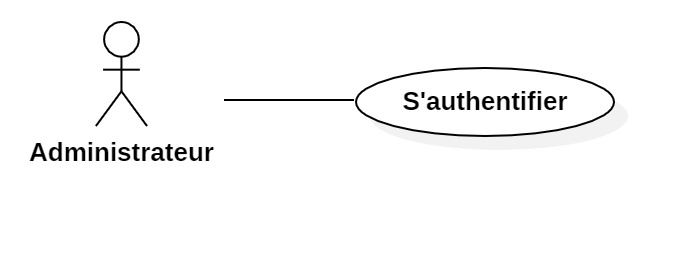
\includegraphics[width=10cm]{images/sauthentifier.jpg}}
     \caption{Diagramme du cas d'utilisation <<S'authentifier>>}
     \label{fig:auth_diagram}
\end{figure}\\
Le tableau \ref{tab:rafLogin} illustre la description détaillée du cas d'utilisation `s’authentifier`.
\begin{table}[!h]
\centering
\caption{Description textuelle du cas d’utilisation «S’authentifier»}
\renewcommand{\arraystretch}{1.2}
\begin{tabular}{|p{4.2cm}|p{11cm}|}
\hline
\textbf{Cas d'utilisation} & S'authentifier \\
\hline
\textbf{Acteur} & Utilisateur \\
\hline
\textbf{Pré-conditions} & Système en marche, utilisateur inscrit \\
\hline
\textbf{Post-conditions} & Utilisateur authentifié, redirigé selon son rôle \\
\hline
\textbf{Scénario de base} & 
1. Affichage de l’interface de connexion \newline
2. Saisie de l’email et du mot de passe \newline
3. Clic sur « Se connecter » \newline
4. Vérification des identifiants \newline
5. Redirection vers l’accueil \\
\hline
\textbf{Exceptions} & 
- Erreur si identifiants incorrects \newline
- Redirection vers l’authentification si le token JWT est expiré \\
\hline
\end{tabular}
\label{tab:rafLogin}
\end{table}
\newpage
\subsection{Raffinement du cas d'utilisation <<Se déconnecter>>}
La figure~\ref{fig:logout_diagram} illustre le diagramme de cas d’utilisation « Se déconnecter ».

\begin{figure}[h]
     \centering
     \fbox{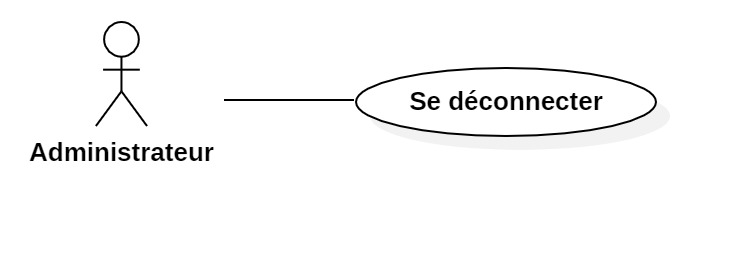
\includegraphics[width=11cm]{images/deconn.jpg}}
     \caption{Diagramme du cas d'utilisation <<Se déconnecter>>}
     \label{fig:logout_diagram}
\end{figure}
Le tableau \ref{tab:rafLogout} illustre la description détaillée du cas d'utilisation `Se déconnecter`.
\begin{table}[!h]
\centering
\caption{Cas d’utilisation : Se déconnecter}
\renewcommand{\arraystretch}{1.2}
\begin{tabular}{|p{4.2cm}|p{11cm}|}
\hline
\textbf{Cas d'utilisation} & Se déconnecter \\
\hline
\textbf{Acteur} & Utilisateur \\
\hline
\textbf{Pré-conditions} & Système en marche, utilisateur connecté \\
\hline
\textbf{Post-conditions} & Utilisateur déconnecté \\
\hline
\textbf{Scénario de base} & 
1. L’utilisateur clique sur « Se déconnecter » \newline
2. Le système redirige vers l’interface d’authentification \\
\hline
\textbf{Exceptions} & 
- Échec de déconnection (erreur API) \\
\hline
\end{tabular}
\label{tab:rafLogout}
\end{table}
\subsection{Raffinement du cas d'utilisation <<Gérer les utilisateurs>>}
La figure~\ref{fig:manage_users_diagram} illustre le diagramme de cas d'utilisation « Gérer les utilisateurs ».

\begin{figure}[h]
     \centering
     \fbox{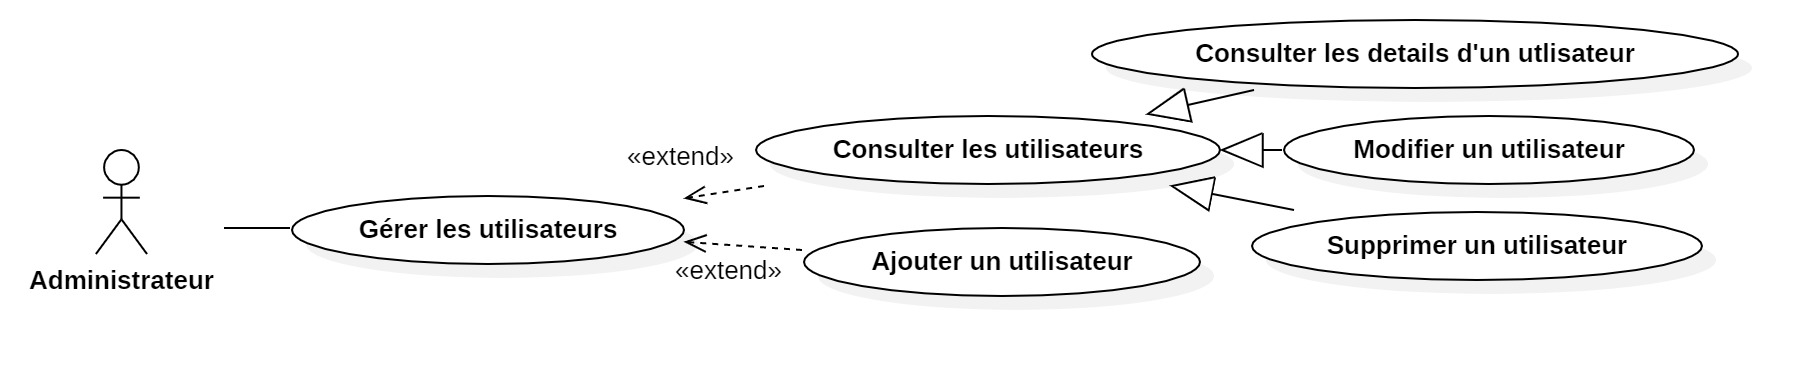
\includegraphics[width=17cm]{images/gererUsers.jpg}}
     \caption{Diagramme du cas d'utilisation <<Gérer les utilisateurs>>}
     \label{fig:manage_users_diagram}
\end{figure}
\newpage
Le tableau~\ref{tab:add_user} illustre la description détaillée du cas d'utilisation « Ajouter un utilisateur ».

\begin{table}[!ht]
\centering
\caption{Description textuelle du cas d’utilisation « Ajouter un utilisateur »}
\label{tab:add_user}
\renewcommand{\arraystretch}{1.2}
\begin{tabular}{|p{4.2cm}|p{11cm}|}
\hline
\textbf{Cas d'utilisation} & Ajouter un utilisateur \\
\hline
\textbf{Acteur} & Admin \\
\hline
\textbf{Pré-conditions} & Le système est en marche. \newline L’admin est authentifié. \\
\hline
\textbf{Post-conditions} & L'utilisateur est ajouté. \\
\hline
\textbf{Scénario de base} & 
1. Le système affiche l’interface d’ajout. \newline
2. L’admin saisit les données du nouvel utilisateur (nom, email, rôle, etc.). \newline
3. L’admin clique sur le bouton « Ajouter ». \newline
4. Le système enregistre les informations. \newline
5. Le système affiche un message de succès. \\
\hline
\textbf{Exceptions} & 
Échec d’ajout (entrées invalides, problème avec l’API POST, ou erreur de base de données). \\
\hline
\end{tabular}
\end{table}


Le tableau~\ref{tab:view_users} illustre la description détaillée du cas d'utilisation « Consulter les utilisateurs ».

\begin{table}[!ht]
\centering
\caption{Description textuelle du cas d’utilisation « Consulter les utilisateurs »}
\label{tab:view_users}
\renewcommand{\arraystretch}{1.2}
\begin{tabular}{|p{4.2cm}|p{11cm}|}
\hline
\textbf{Cas d'utilisation} & Consulter les utilisateurs \\
\hline
\textbf{Acteur} & Admin \\
\hline
\textbf{Pré-conditions} & Le système est en marche. \newline L’admin est authentifié. \\
\hline
\textbf{Post-conditions} & La liste des utilisateurs est consultée. \\
\hline
\textbf{Scénario de base} & 
1. Le système affiche la liste des utilisateurs. \newline
2. L’admin consulte la liste. \\
\hline
\textbf{Exceptions} & 
Échec de consultation (problème avec l’API GET, ou erreur de base de données). \\
\hline
\textbf{Extensions} & 
Modifier un utilisateur. \newline Supprimer un utilisateur. \\
\hline
\end{tabular}
\end{table}

\newpage
Le tableau~\ref{tab:view_user_details} illustre la description détaillée du cas d'utilisation « Consulter les détails d’un utilisateur ».

\begin{table}[!ht]
\centering
\caption{Description textuelle du cas d’utilisation « Consulter les détails d’un utilisateur »}
\label{tab:view_user_details}
\renewcommand{\arraystretch}{1.2}
\begin{tabular}{|p{4.2cm}|p{11cm}|}
\hline
\textbf{Cas d'utilisation} & Consulter les détails d’un utilisateur \\
\hline
\textbf{Acteur} & Admin \\
\hline
\textbf{Pré-conditions} & Le système est en marche. \newline L’admin est authentifié. \\
\hline
\textbf{Post-conditions} & Les informations détaillées de l’utilisateur sont affichées. \\
\hline
\textbf{Scénario de base} & 
1. L’admin clique sue le bouton pour afficher les détails d'un utilisateur depuis la liste. \newline
2. Le système affiche les informations détaillées de l’utilisateur (nom, email, rôle, date de création, etc.). \\
\hline
\textbf{Exceptions} & 
Échec de consultation (problème avec l’API GET, ou erreur de base de données). \\
\hline
\end{tabular}
\end{table}
\vspace{0.5cm}
Le tableau~\ref{tab:update_user} illustre la description détaillée du cas d'utilisation « Modifier un utilisateur ».

\begin{table}[!ht]
\centering
\caption{Description textuelle du cas d’utilisation « Modifier un utilisateur »}
\label{tab:update_user}
\renewcommand{\arraystretch}{1.2}
\begin{tabular}{|p{4.2cm}|p{11cm}|}
\hline
\textbf{Cas d'utilisation} & Modifier un utilisateur \\
\hline
\textbf{Acteur} & Admin \\
\hline
\textbf{Pré-conditions} & Le système est en marche. \newline L’admin est authentifié. \\
\hline
\textbf{Post-conditions} & L'utilisateur est modifié. \\
\hline
\textbf{Scénario de base} & 
1. Le système affiche l’interface de modification. \newline
2. L’admin saisit les nouvelles données. \newline
3. L’admin clique sur le bouton « Modifier ». \newline
4. Le système enregistre les modifications. \newline
5. Le système affiche un message de succès. \\
\hline
\textbf{Exceptions} & 
Échec de modification (problème avec l’API PUT, ou erreur de base de données). \\
\hline
\end{tabular}
\end{table}

\newpage
\vspace*{-1.5cm}
Le tableau~\ref{tab:delete_user} illustre la description détaillée du cas d'utilisation « Supprimer un utilisateur ».

\begin{table}[!ht]
\centering
\caption{Description textuelle du cas d’utilisation « Supprimer un utilisateur »}
\label{tab:delete_user}
\renewcommand{\arraystretch}{1.2}
\begin{tabular}{|p{4.2cm}|p{11cm}|}
\hline
\textbf{Cas d'utilisation} & Supprimer un utilisateur \\
\hline
\textbf{Acteur} & Admin \\
\hline
\textbf{Pré-conditions} & Le système est en marche. \newline L’admin est authentifié. \\
\hline
\textbf{Post-conditions} & L'utilisateur est supprimé. \\
\hline
\textbf{Scénario de base} & 
1. L’admin clique sur le bouton « Supprimer » d’un utilisateur. \newline
2. Le système supprime les données correspondantes. \newline
3. Le système affiche un message de succès. \\
\hline
\textbf{Exceptions} & 
Échec de suppression (problème avec l’API DELETE, ou erreur de base de données). \\
\hline
\end{tabular}
\end{table}
\subsection{Raffinement du cas d'utilisation <<Mise en place et configuration de Camunda>>}
Le tableau~\ref{tab:confCamunda} illustre la description détaillée du cas d'utilisation « Mise en place et configuration de Camunda ».
\begin{table}[!h]
\centering
\caption{Description textuelle du cas d’utilisation «Mise en place et configuration de Camunda»}
\label{tab:confCamunda}
\renewcommand{\arraystretch}{1.2}
\begin{tabular}{|p{4.2cm}|p{11cm}|}
\hline
\textbf{Cas d'utilisation} & Mise en place et configuration de Camunda \\
\hline
\textbf{Acteur} & Développeur \\
\hline
\textbf{Pré-conditions} & 
Le projet backend (Spring Boot) est accessible. \newline
L’environnement de développement est configuré (Java, Maven, IDE). \\
\hline
\textbf{Post-conditions} & Le moteur Camunda est intégré, configuré et fonctionnel dans l’application Spring Boot. \\
\hline
\textbf{Scénario de base} & 
1. Le développeur identifie la version de Camunda compatible avec la version de Spring Boot utilisée dans le projet. \newline
2. Le développeur ajoute les dépendances Camunda nécessaires dans le fichier \texttt{pom.xml}. \newline
3. Le développeur configure les propriétés Camunda dans le fichier \texttt{application.properties}. \newline
4. Le développeur initialise et configure le moteur de workflow dans la classe de configuration Spring. \newline
5. Le développeur crée un processus BPMN simple pour tester l’intégration. \newline
6. Le système valide le bon fonctionnement du moteur. \\
\hline
\textbf{Exceptions} & 
Erreurs d’intégration : dépendances manquantes, mauvaise configuration, problèmes de base de données ou de compatibilité. \\
\hline
\end{tabular}
\end{table}
\newpage
\section{Conception}
La conception est une phase importante pour la bonne réalisation d'un projet.Dans cette partie nous allons exposer la conception des cas d'utilisations de ce sprint qui se traduit par un diagramme de classe globale de ce sprint suivi par les diagrammes de classes et les diagrammes de séquences de chaque cas d'utilisation.
\subsection{Diagramme de classe du sprint 1}
La figure~\ref{fig:class_diagram_sprint1} illustre le diagramme de classe du Sprint 1. Il est formé de :
\begin{itemize}
    \item \textbf{Classe "Permission"} : C’est une énumération qui définit les permissions des différents rôles (ADMIN, MANAGER, etc.).
    \item \textbf{Classe "Role"} : C’est une énumération qui permet d’identifier les rôles des utilisateurs de la plateforme.
    \item \textbf{Classe "Token"} : C’est la classe qui gère les jetons d’authentification des utilisateurs.
    \item \textbf{Classe "User"} : C’est la classe qui représente tous les utilisateurs ayant accès à la plateforme.
    \item \textbf{Interface "Implements Spring Security UserDetails"} : Indique que la classe User implémente cette interface pour gérer l’authentification et l’autorisation.
\end{itemize}
\begin{figure}[h]
     \centering
     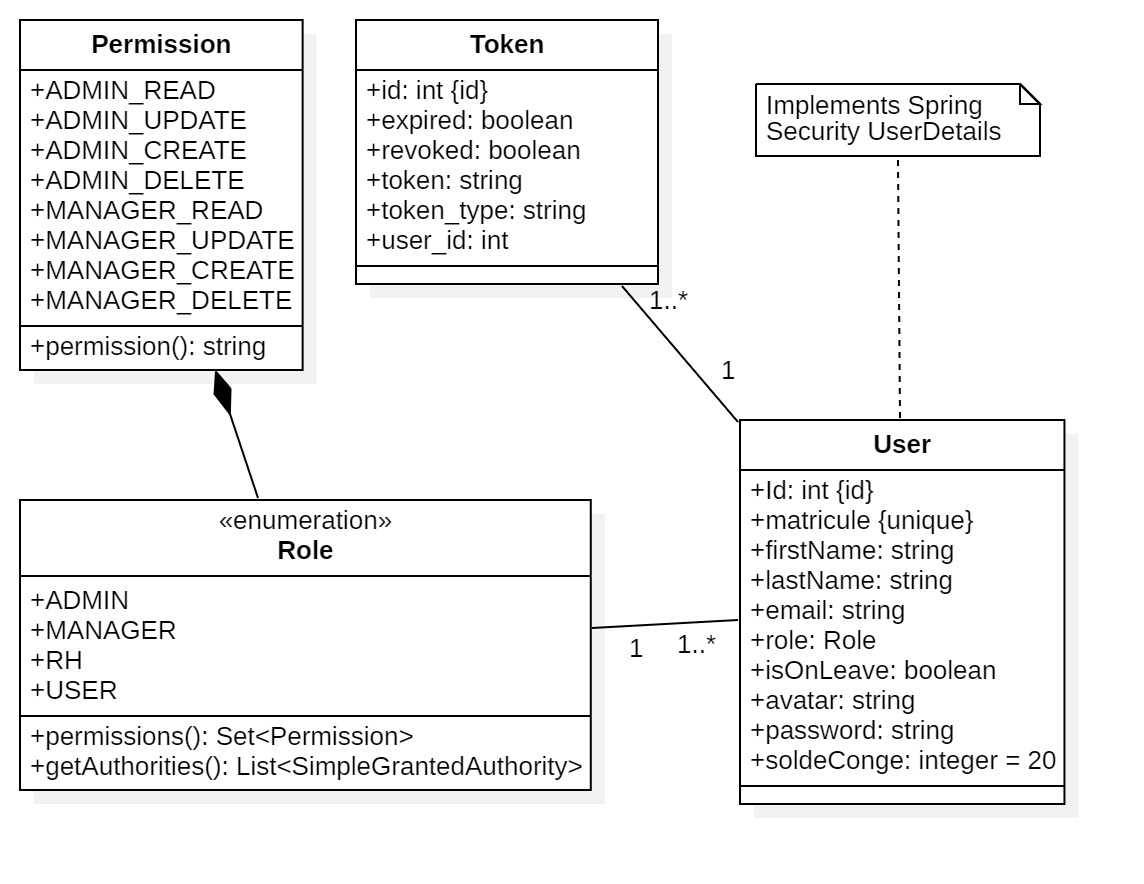
\includegraphics[width=12cm]{images/ClassDiagUs.jpg}
     \caption{Diagramme de classe du sprint 1}
     \label{fig:class_diagram_sprint1}
 \end{figure}
 \newpage
 \subsection{Conception du cas d'utilisation «S'authentifier»}
\subsubsection{Diagramme de classe}
La figure \ref{fig:cauth} illustre le diagramme de classes du cas d’utilisation s'authentifier.
\begin{figure}[h]
     \centering
      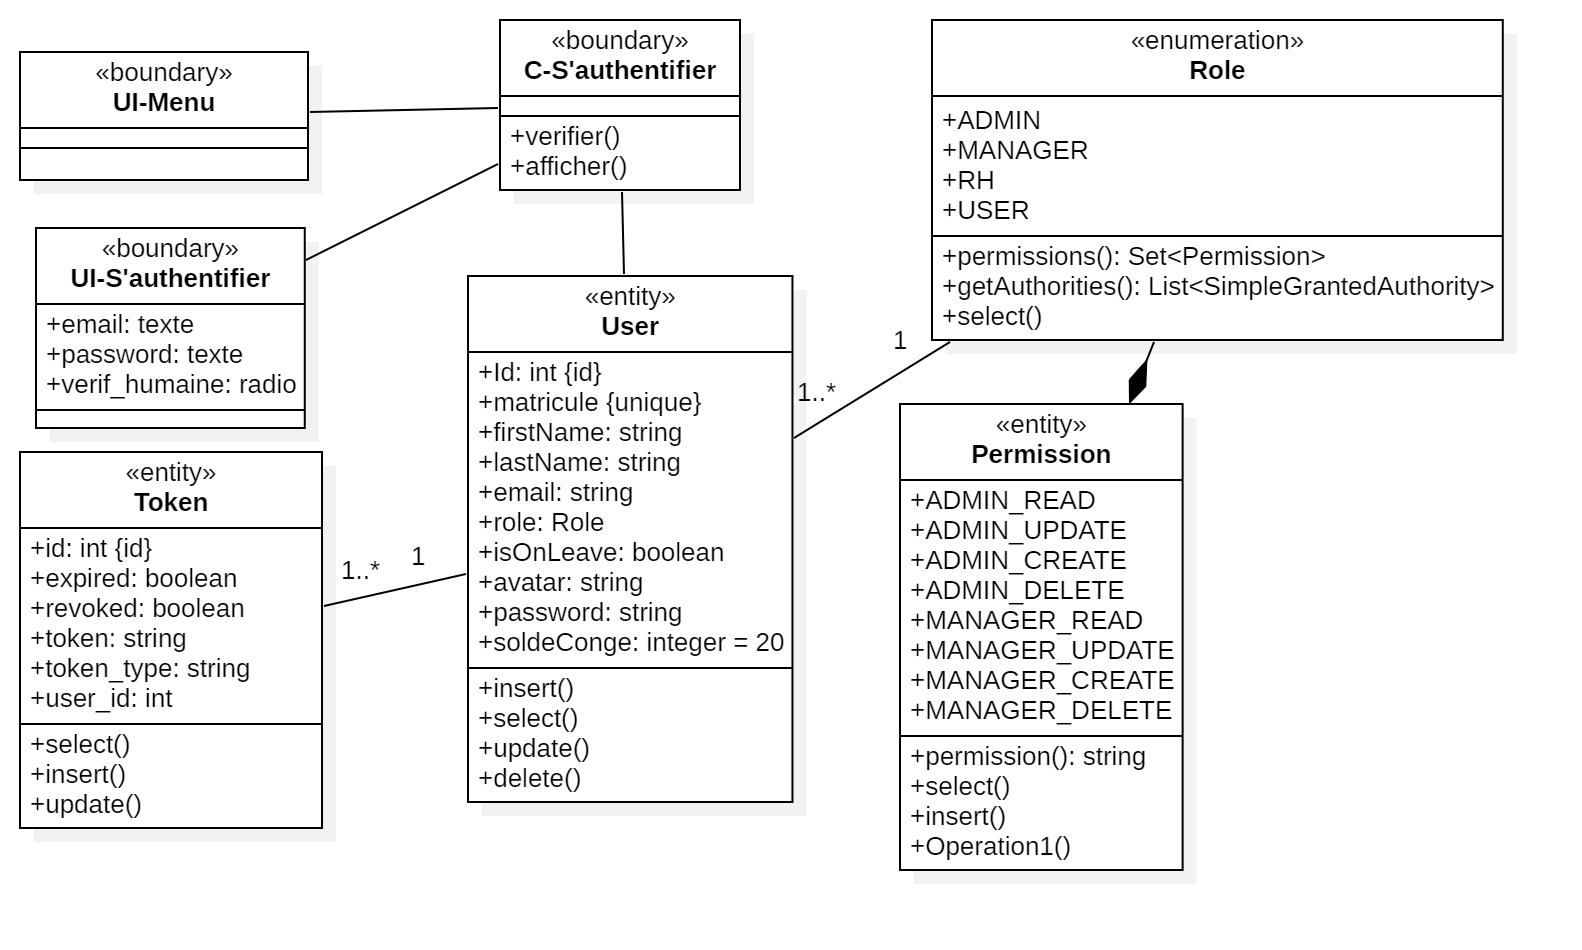
\includegraphics[width=17cm]{images/C-S'authentifier.jpg}
     \caption{Diagramme de classe du cas d'utilisation <<S'authentifier>>}
     \label{fig:cauth}
 \end{figure}
 \subsubsection{Diagramme de séquence}
Au lancement de l'application, une interface d'authentification apparaîtra. Ensuite, les utilisateurs peuvent entrer leurs adresses mail et mots de passe, et vérifier qu'ils ne sont pas un robot (recaptcha), qui seront envoyés via l'interface d'authentification au contrôleur d'authentification, qui à son tour vérifie les informations dans l'entité \textit{Utilisateur}.\\
Si les coordonnées sont correctes, ils seront amenés à un espace approprié selon leurs rôles. Sinon, un message d'erreur d'authentification sera affiché.\\
\noindent La figure~\ref{fig:sauth} modélise le diagramme de séquence du cas d'utilisation « S'authentifier ».
\clearpage
\begin{figure}[h]
     \centering
     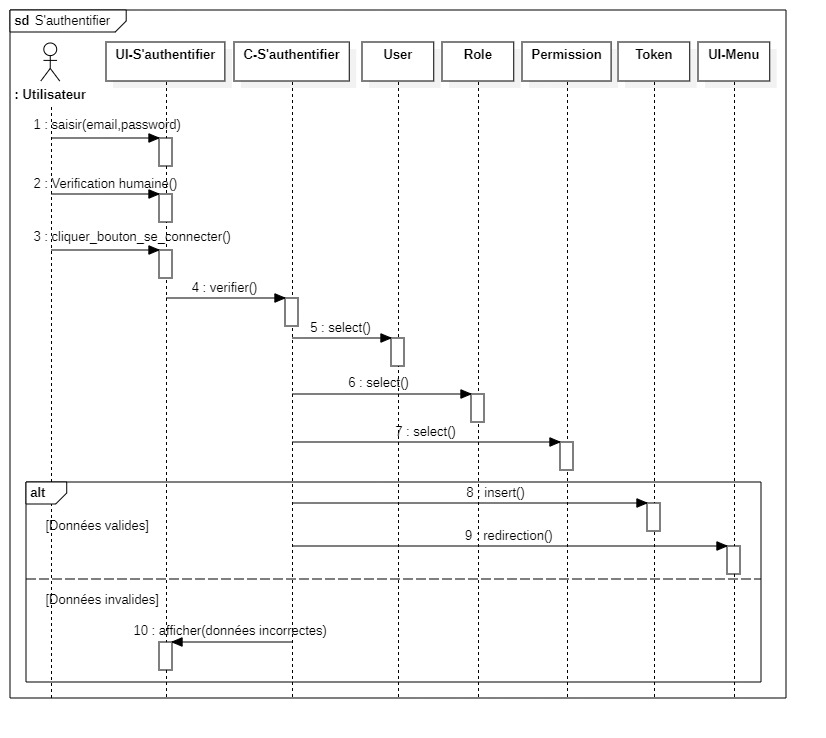
\includegraphics[width=18cm]{images/S-S'authentifier.jpg}
     \caption{Diagramme de séquence du cas d'utilisation <<S'authentifier>>}
     \label{fig:sauth}
\end{figure}

\subsection{Conception du cas d'utilisation «Se déconnecter»}
\subsubsection{Diagramme de classe}
La figure \ref{fig:cdec} illustre le diagramme de classe du cas d’utilisation se déconnecter.
\newpage

\begin{figure}[h]
     \centering
      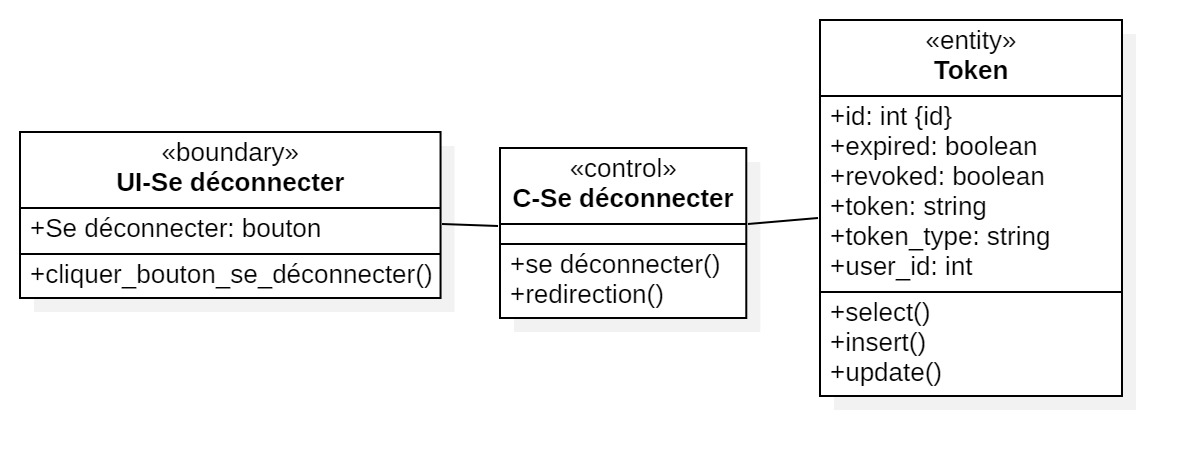
\includegraphics[width=15cm]{images/C-dec.jpg}
     \caption{Diagramme de classe du cas d'utilisation <<Se déconnecter>>}
     \label{fig:cdec}
 \end{figure}
\subsubsection{Diagramme de séquence}
 Si l'utilisateur souhaite se déconnecter, il clique sur le bouton de déconnexion dans le menu. Le système supprime les données obtenues avec l'authentification de l'utilisateur et retire son token. Ce dernier sera finalement redirigé vers l'interface d'authentification.\\
 La figure \ref{fig:sdec} illustre le diagramme de séquence du cas d’utilisation se déconnecter.\\
 \vspace{-0.5cm}
\begin{figure}[h]
     \centering
     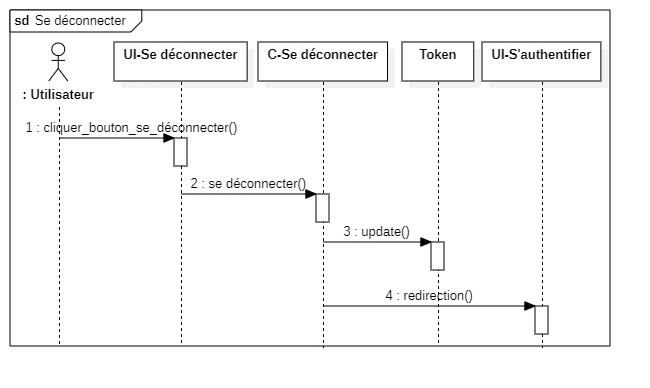
\includegraphics[width=15cm]{images/S-dec.jpg}
     \caption{Diagramme de séquence du cas d'utilisation <<Se déconnecter>>}
     \label{fig:sdec}
\end{figure}
\clearpage
\subsection{Conception du cas d'utilisation «Gérer les utilisateurs»}
\subsubsection{Diagramme de classe}
La figure \ref{fig:cgu} illustre le diagramme de classe du cas d’utilisation gérer les utilisateurs.
\begin{figure}[h]
     \centering
   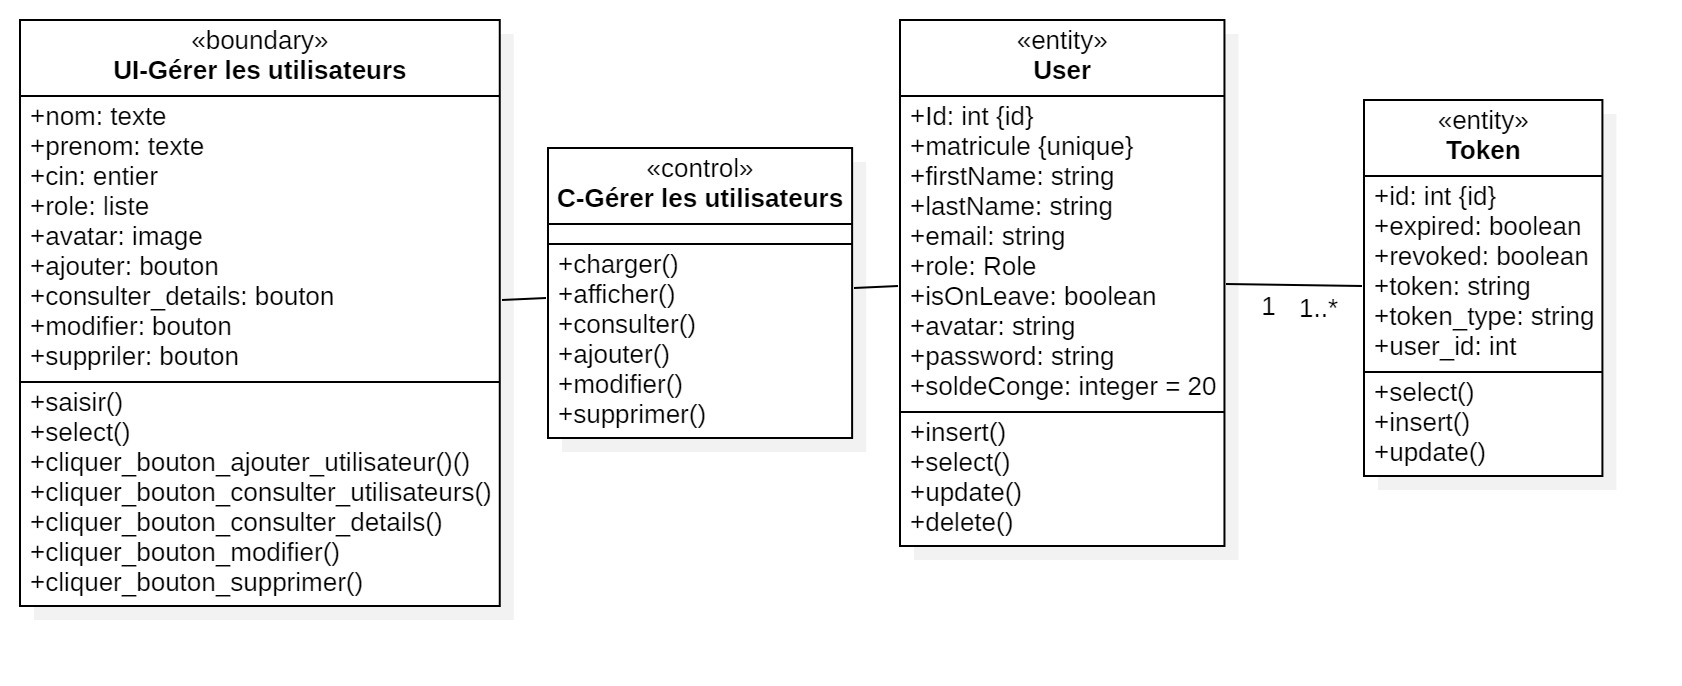
\includegraphics[width=16cm]{images/C-gus.jpg}
     \caption{Diagramme de classe du cas d'utilisation <<Gérer les utilisateurs>>}
     \label{fig:cgu}
 \end{figure}
 \subsubsection{Diagramme de séquence}

Seul l’administrateur dispose des droits nécessaires pour gérer les utilisateurs depuis son interface dédiée. Cette gestion inclut un ensemble d’opérations essentielles telles que l’ajout de nouveaux utilisateurs, la consultation de la liste des utilisateurs existants, l’affichage des détails d’un utilisateur spécifique, la modification de ses informations, ainsi que la suppression d’un compte utilisateur. Toutes ces actions sont déclenchées depuis l’interface d’administration, puis transmises au contrôleur via des requêtes HTTP. Ce dernier assure la logique métier en interagissant avec les entités du système, notamment l’entité "User" pour manipuler les données des utilisateurs, et l’entité "Token" pour révoquer les tokens en cas de suppression d'un utilisateur. \\
La figure~\ref{fig:manage_userss_diagram} illustre le diagramme de séquence du cas d'utilisation « Gérer les utilisateurs ».
\newpage
\vspace*{-3cm} 
\begin{figure}[H]
     \centering
     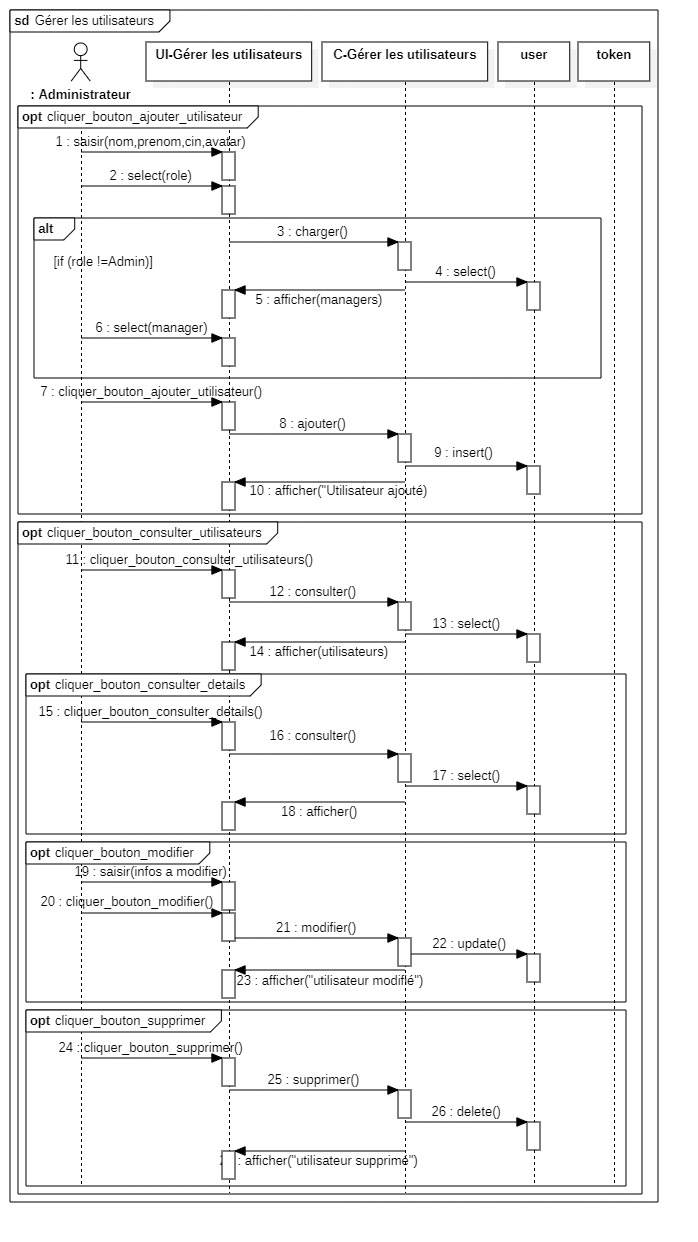
\includegraphics[width=15cm]{images/S-gus.jpg}
     \vspace{-1cm}
     \caption{Diagramme de séquence du cas d'utilisation <<Gérer les utilisateurs>>}
     \label{fig:manage_userss_diagram}
\end{figure}
\section{Réalisation}
Dans cette partie, nous présentons les modules de notre premier sprint en utilisant des captures d’écran.
\subsection{S’authentifier}
L’utilisateur n’est pas autorisé à accéder à l’application, sauf s’il a un compte. Donc, afin d’explorer les fonctionnalités de l’application, l’utilisateur est invité à s’authentifier avec un email et un mot de passe comme le montre la figure \ref{fig:realauth} ci-dessous. L’utilisateur ne peut pas créer un compte puisque les comptes sont attribués par un administrateur.
\begin{figure}[H]
     \centering
     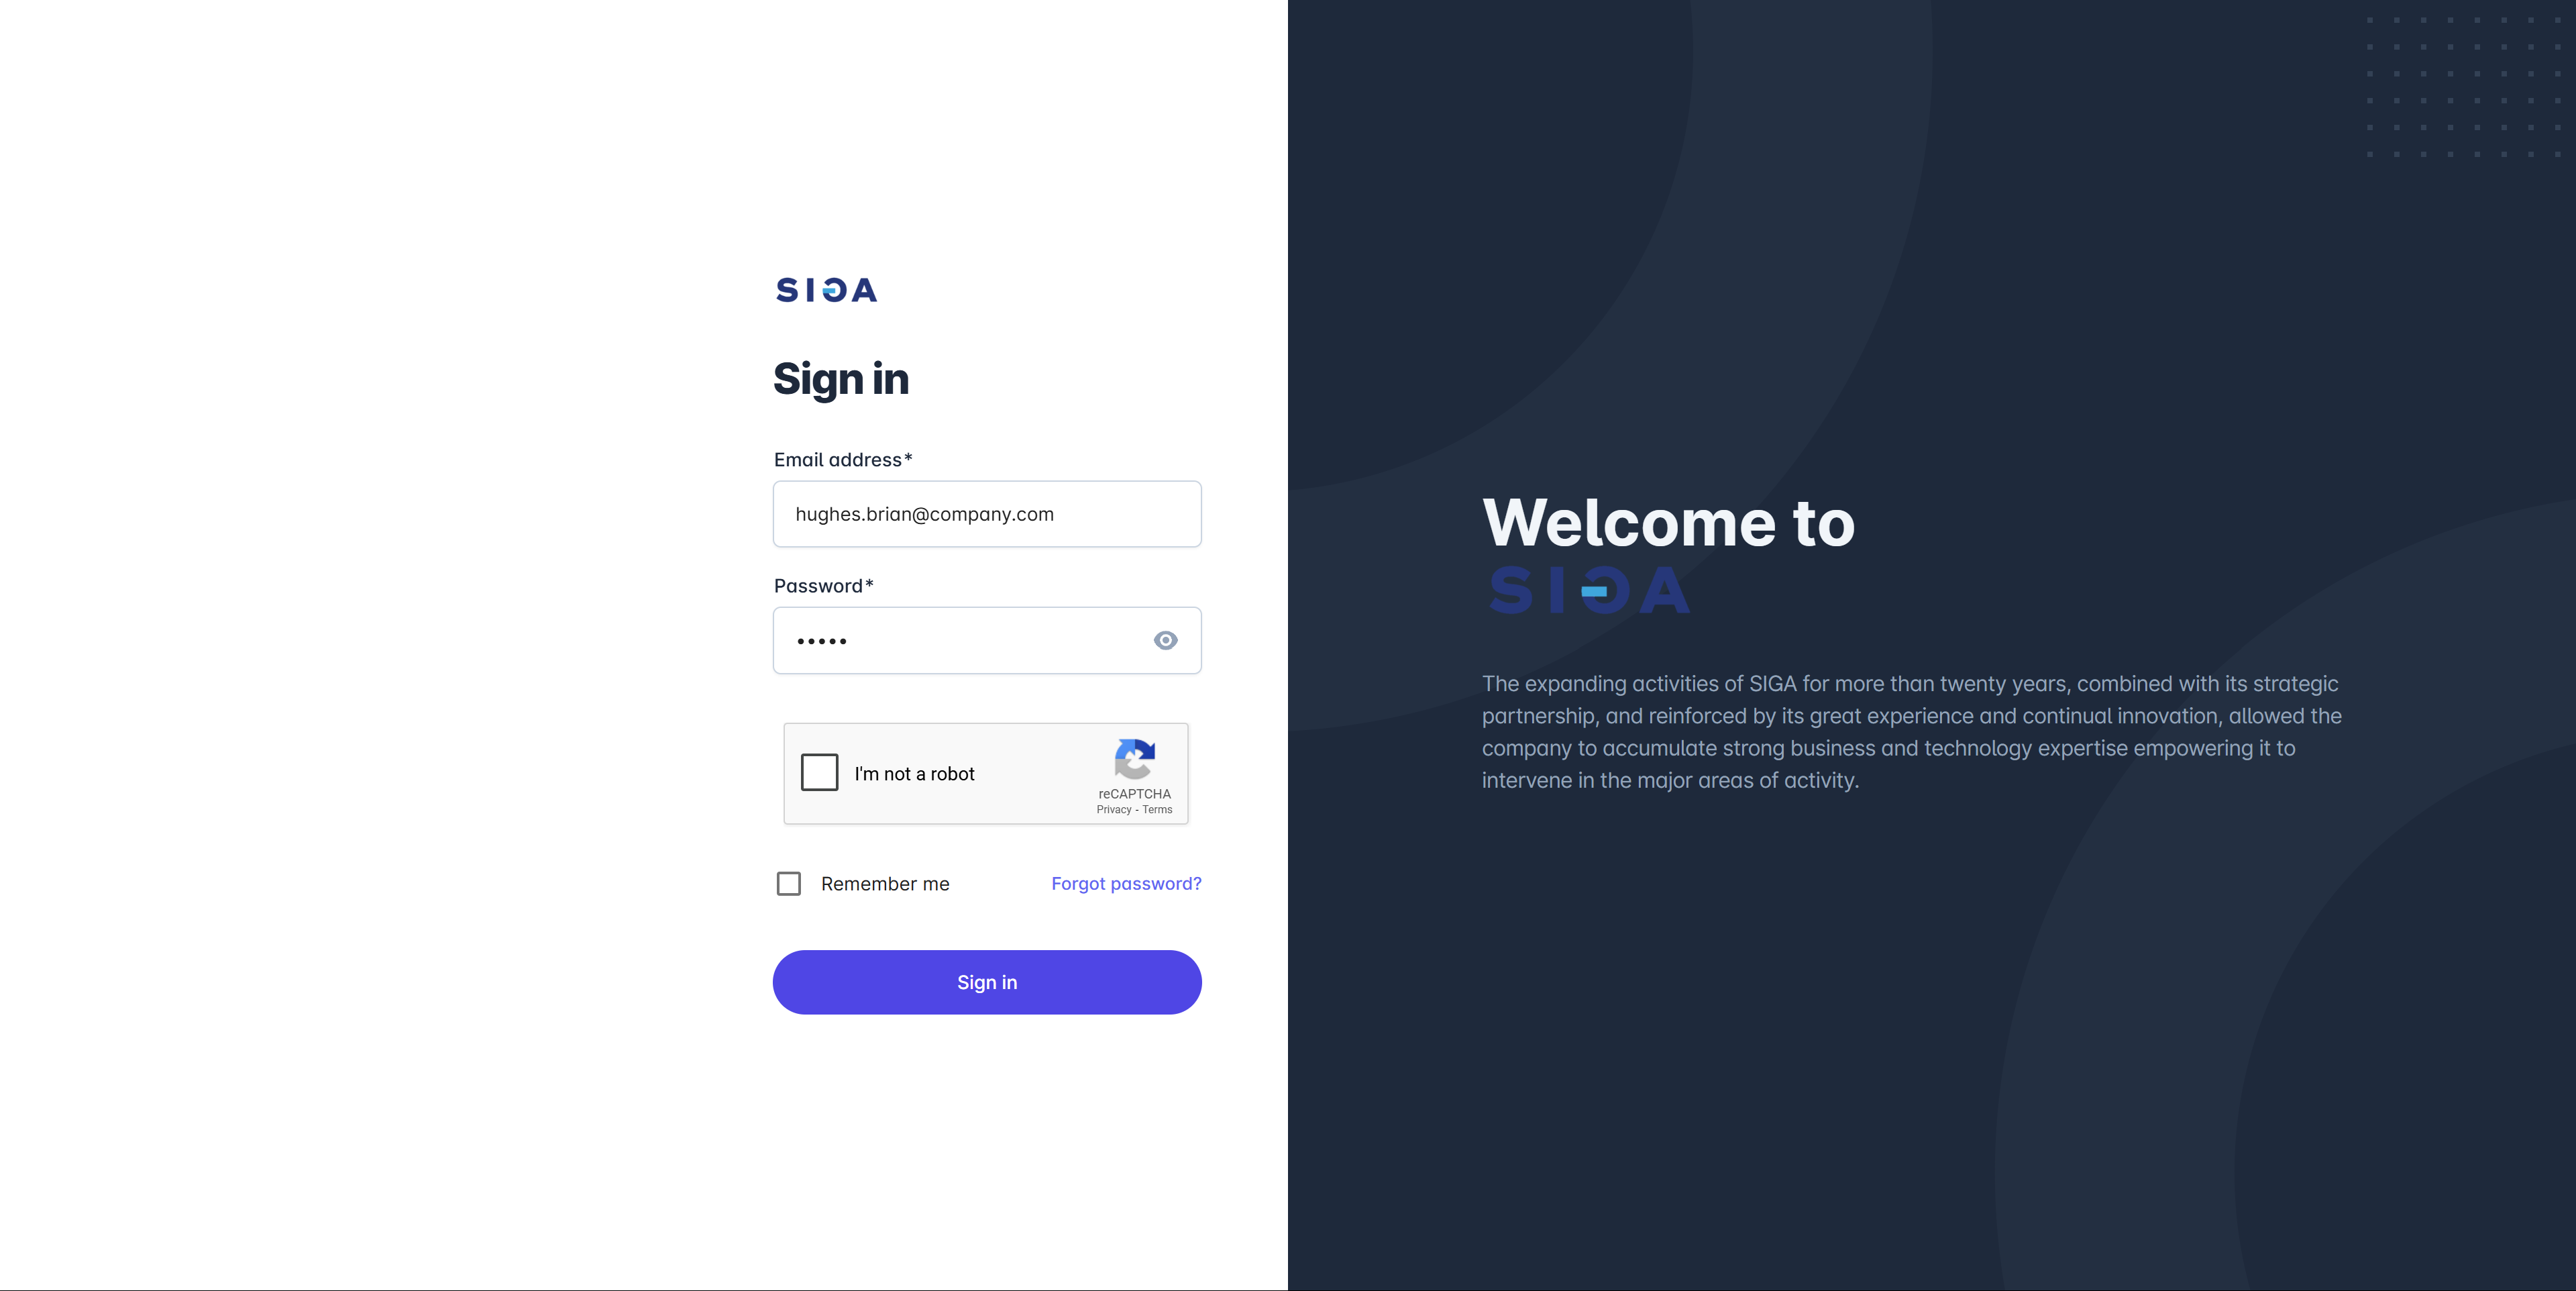
\includegraphics[width=16cm]{images/realisation/login.png}
     \caption{Interface du cas d'utilisation <<S'authentifier>>}
     \label{fig:realauth}
\end{figure}
\subsection{Se déconnecter}
L’utilisateur a la possibilité de se déconnecter de l’application lorsqu’il le souhaite, comme le montre la figure \ref{fig:reallogout}. Cette action met fin à sa session en cours et le redirige vers la page d’authentification.
\newpage
\vspace*{-2cm}
\begin{figure}[H]
     \centering
     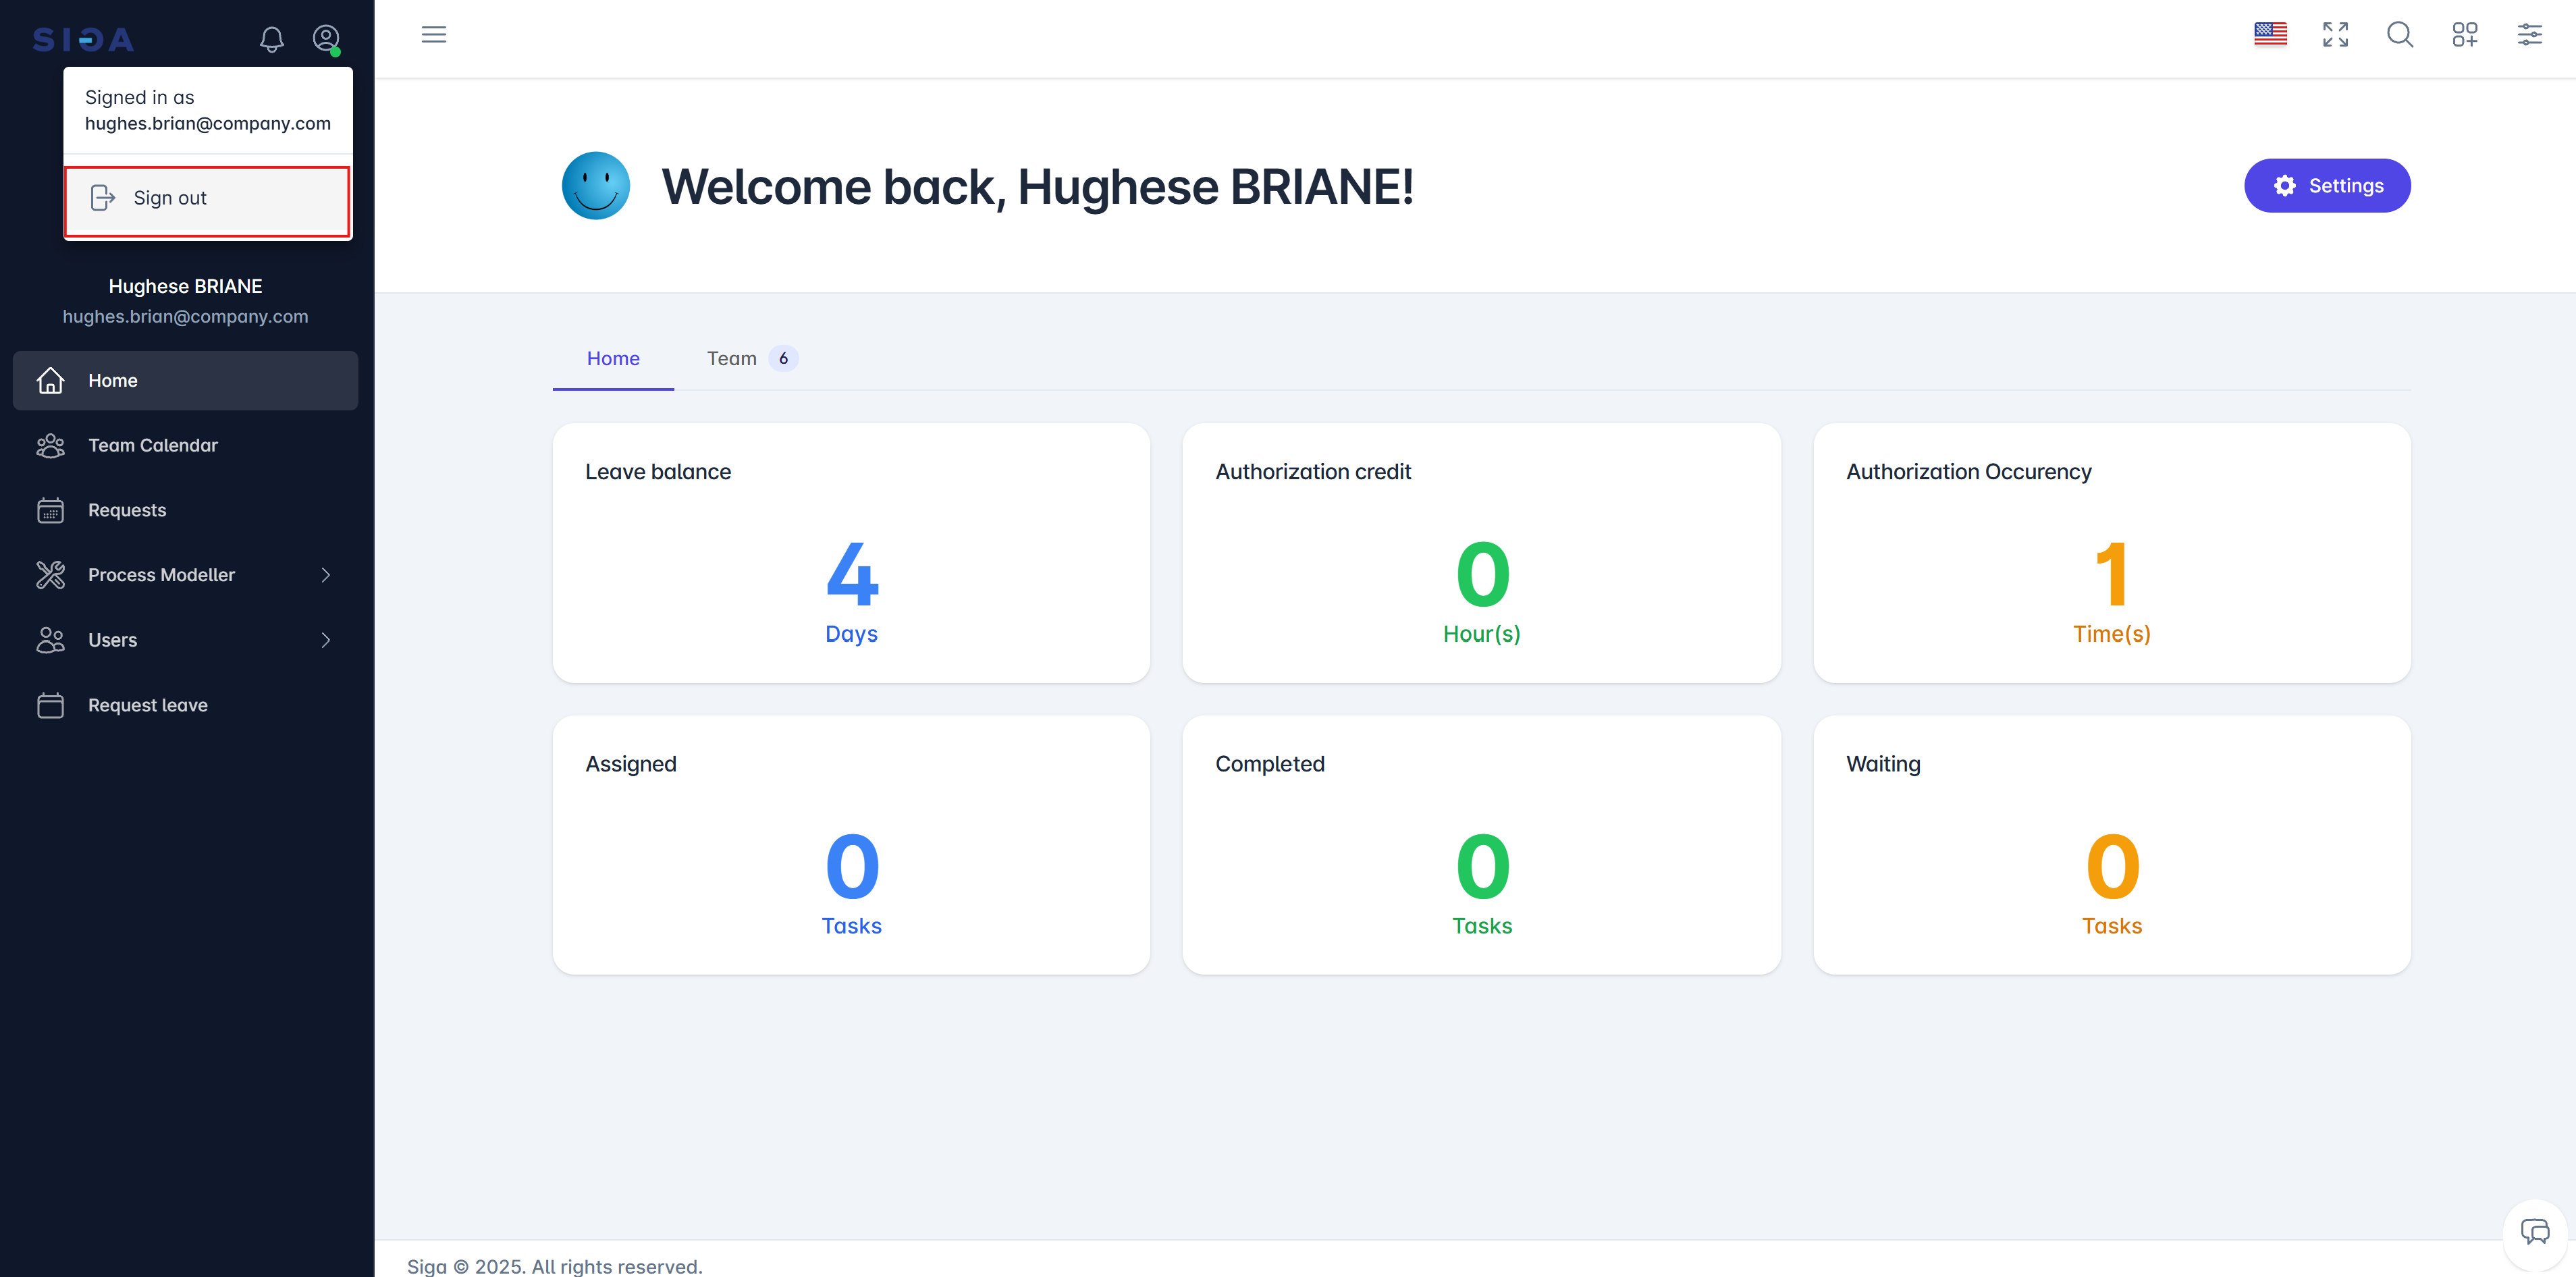
\includegraphics[width=16cm]{images/realisation/decon.png}
     \caption{Interface du cas d'utilisation <<Se déconnecter>>}
     \label{fig:reallogout}
\end{figure}
\subsection{Gérer les utilisateurs}
La gestion des utilisateurs permet à l’administrateur de consulter,ajouter,modifier, supprimer et consulter les détails des utilisateurs.
\subsubsection{Ajouter un utilisateur}
L'administrateur peut ajouter un nouvel utilisateur à l’application via l’interface dédiée accessible depuis le menu latéral, comme illustré dans la figure \ref{fig:adduser}. Il lui suffit de renseigner les informations demandées telles que le prénom, le nom, l’adresse e-mail, le mot de passe, le rôle ainsi qu’un avatar, puis de cliquer sur Create account pour finaliser l’ajout.
\begin{figure}[H]
     \centering
     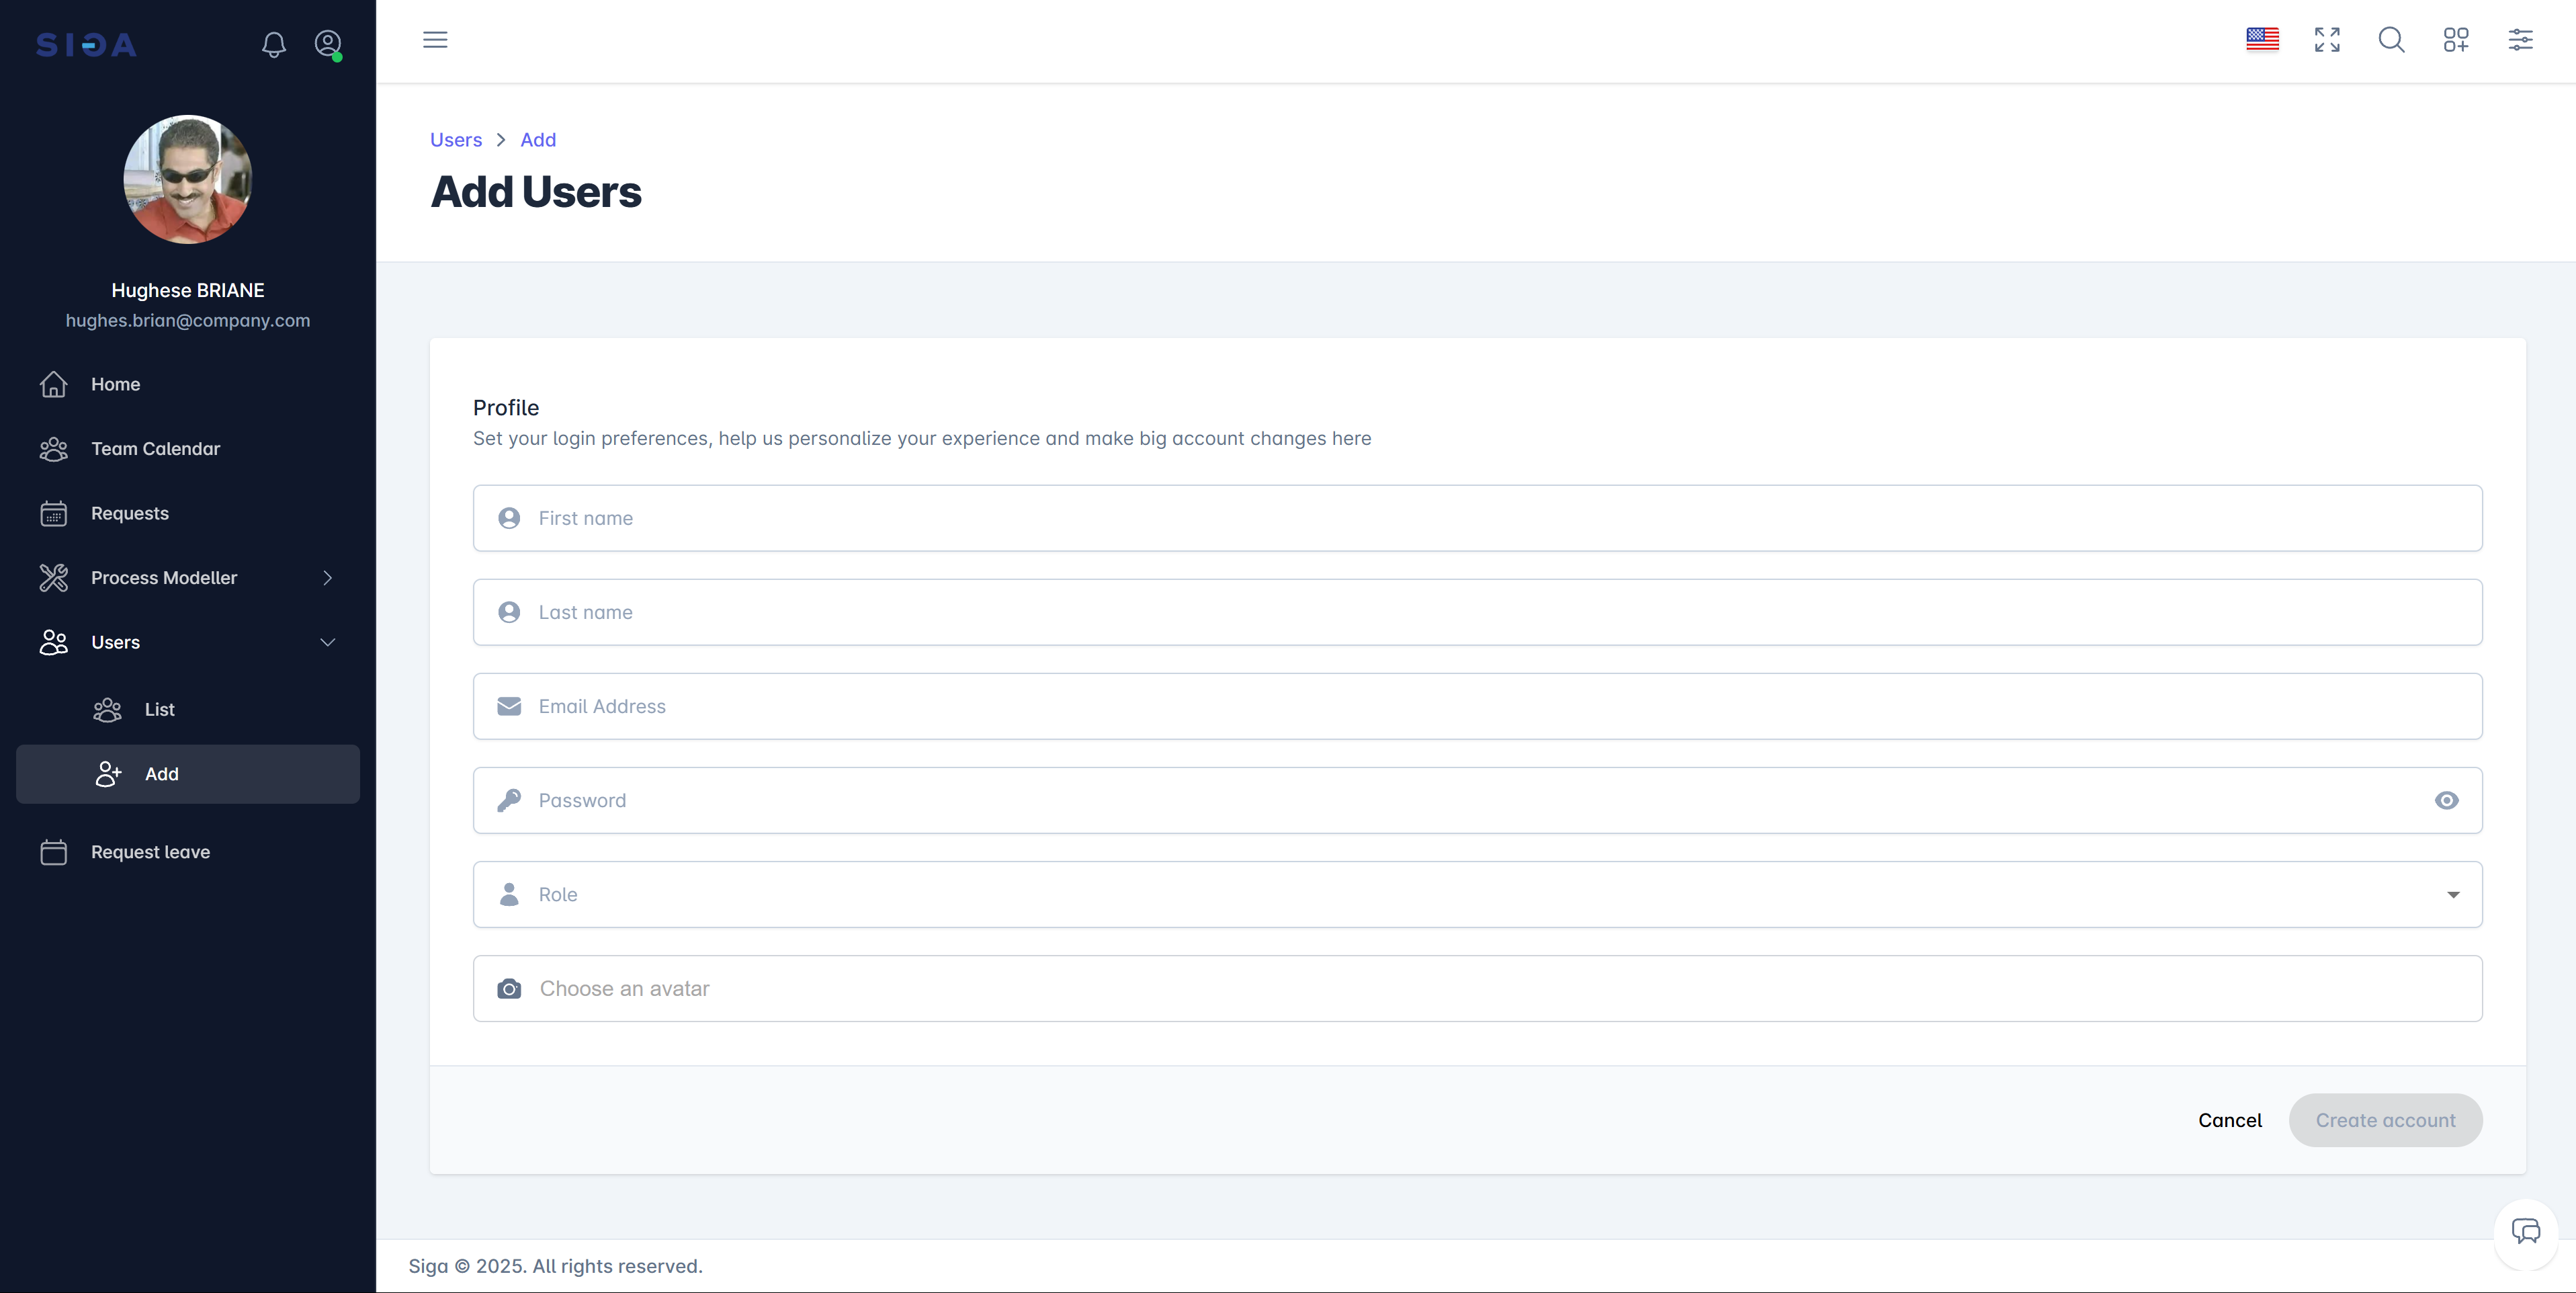
\includegraphics[width=15cm]{images/realisation/addUser.png}
     \caption{Interface du cas d'utilisation <<Ajouter un utilisateur>>}
     \label{fig:adduser}
\end{figure}
\newpage
\subsubsection{Consulter les utilisateurs}
L’administrateur peut consulter la liste des utilisateurs existants via l’onglet Users > List dans le menu latéral, comme le montre la figure \ref{fig:viewusers}. Cette interface permet d’avoir un aperçu global des comptes enregistrés, incluant leurs informations de profil et leur rôle dans le système.
\begin{figure}[H]
     \centering
     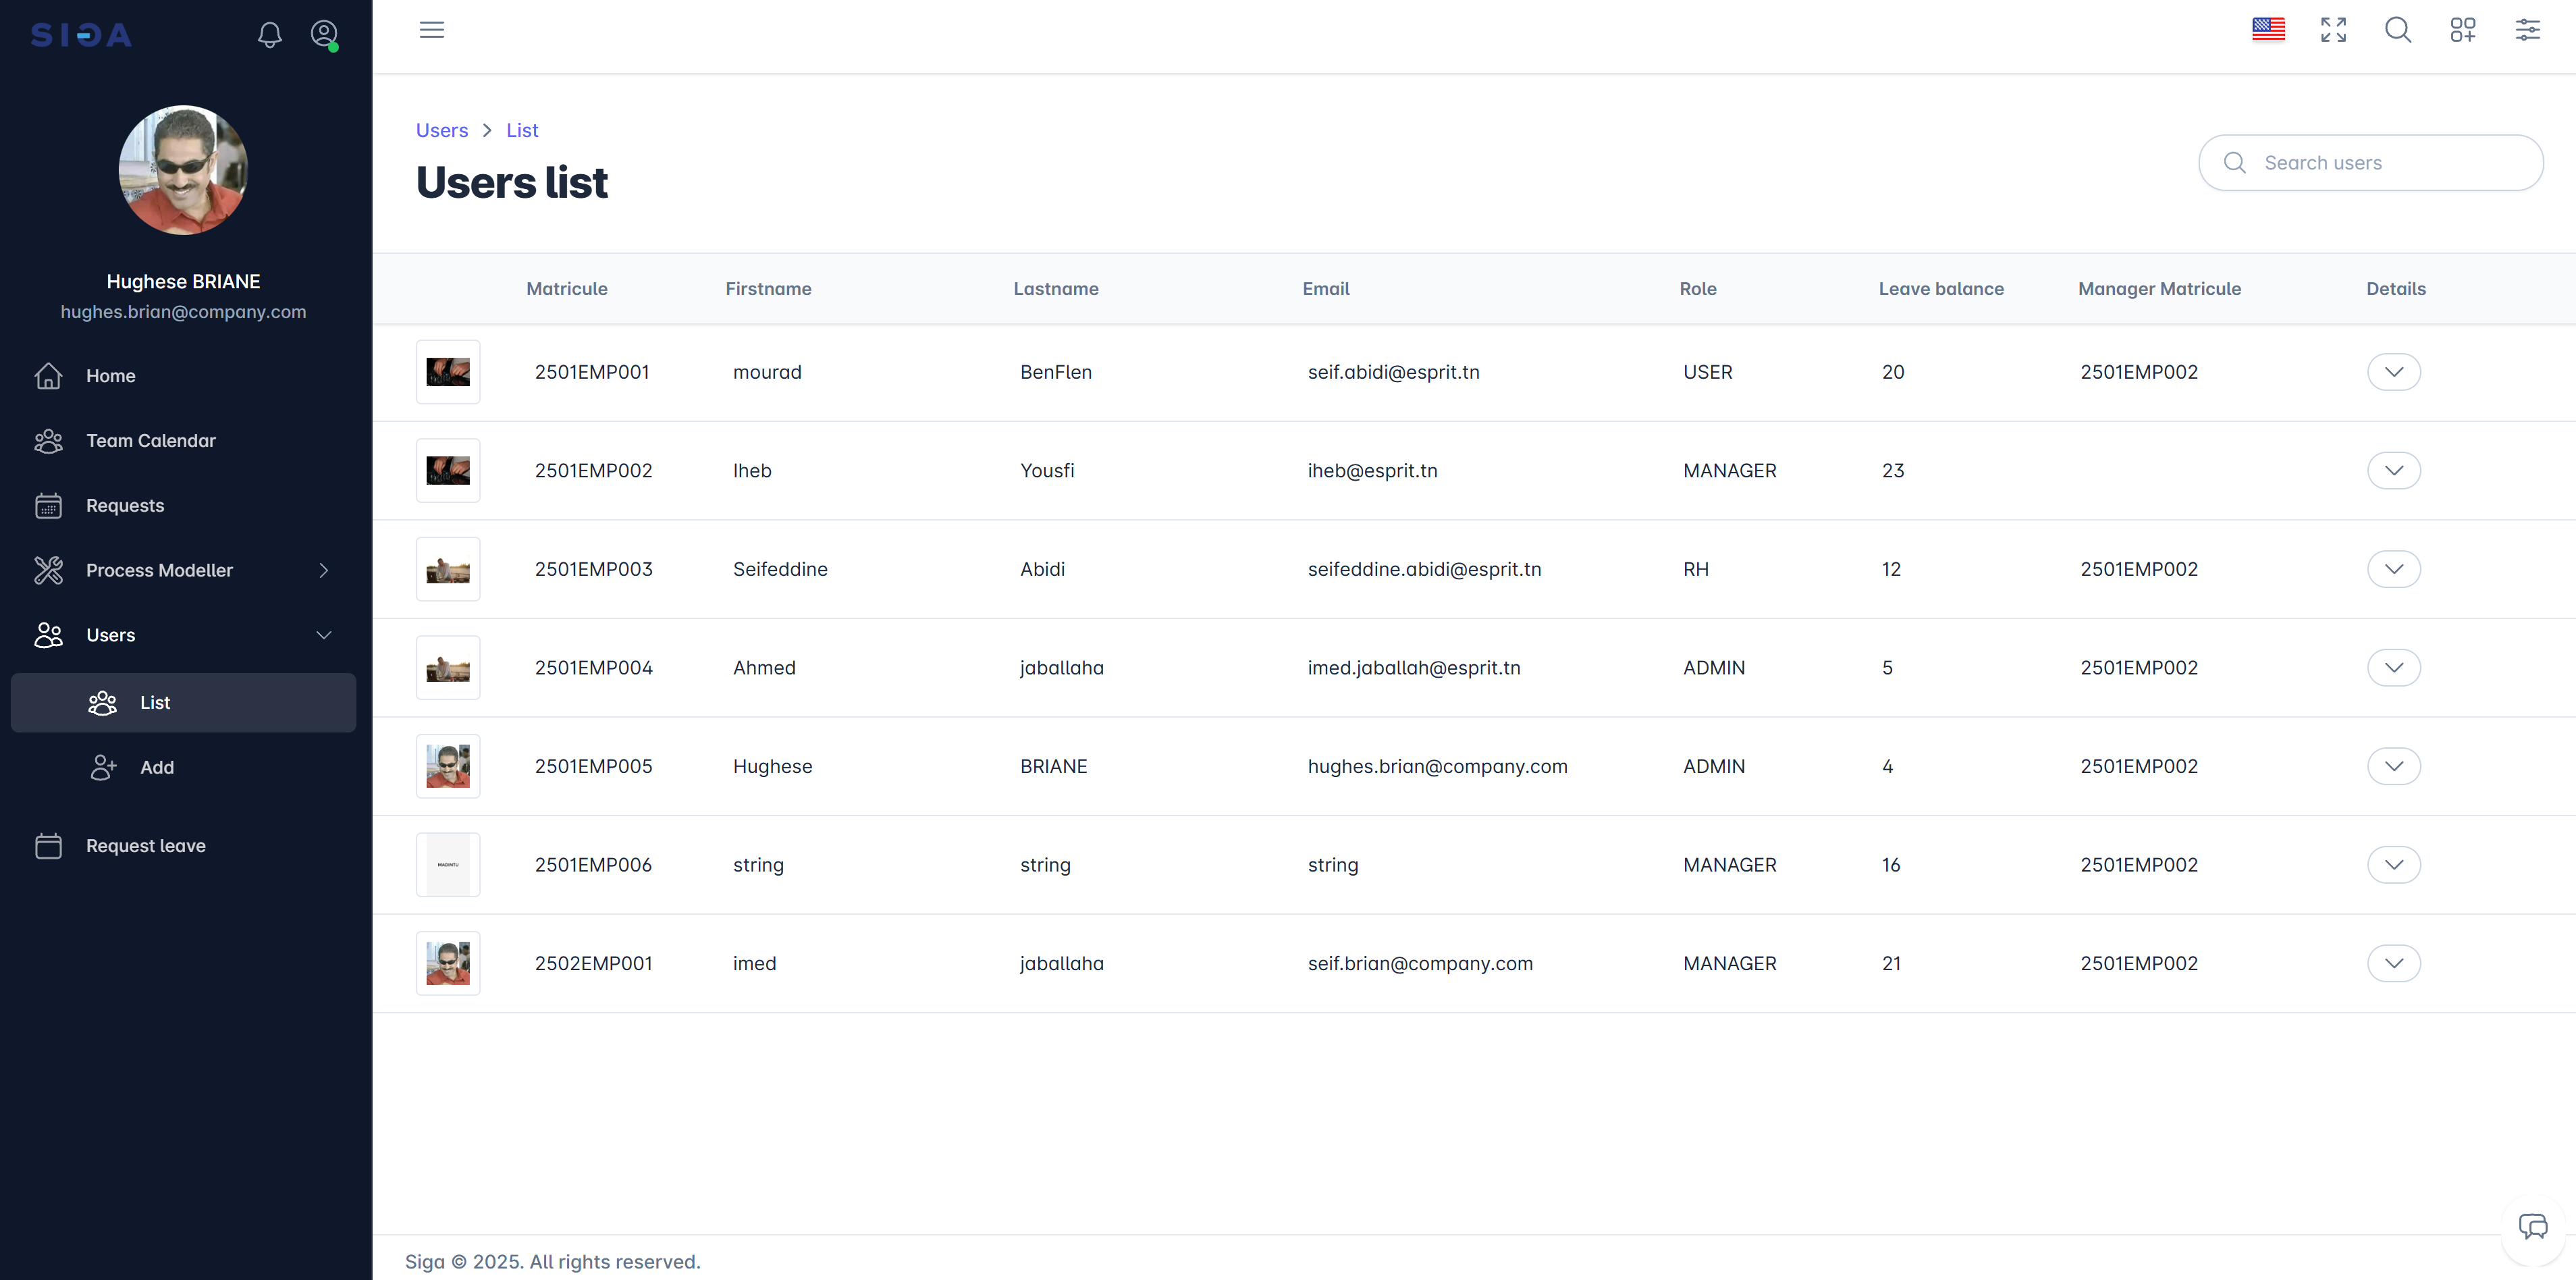
\includegraphics[width=16cm]{images/realisation/vUser.png}
     \caption{Interface du cas d'utilisation <<Consulter les utilisateurs>>}
     \label{fig:viewusers}
\end{figure}
\subsubsection{Consulter les détails d'un utilisateur}
L’administrateur peut consulter les détails d’un compte spécifique en sélectionnant un utilisateur dans la liste, comme illustré dans la figure \ref{fig:userdetails}. Cette action affiche les informations complètes du profil sélectionné.
\begin{figure}[H]
     \centering
     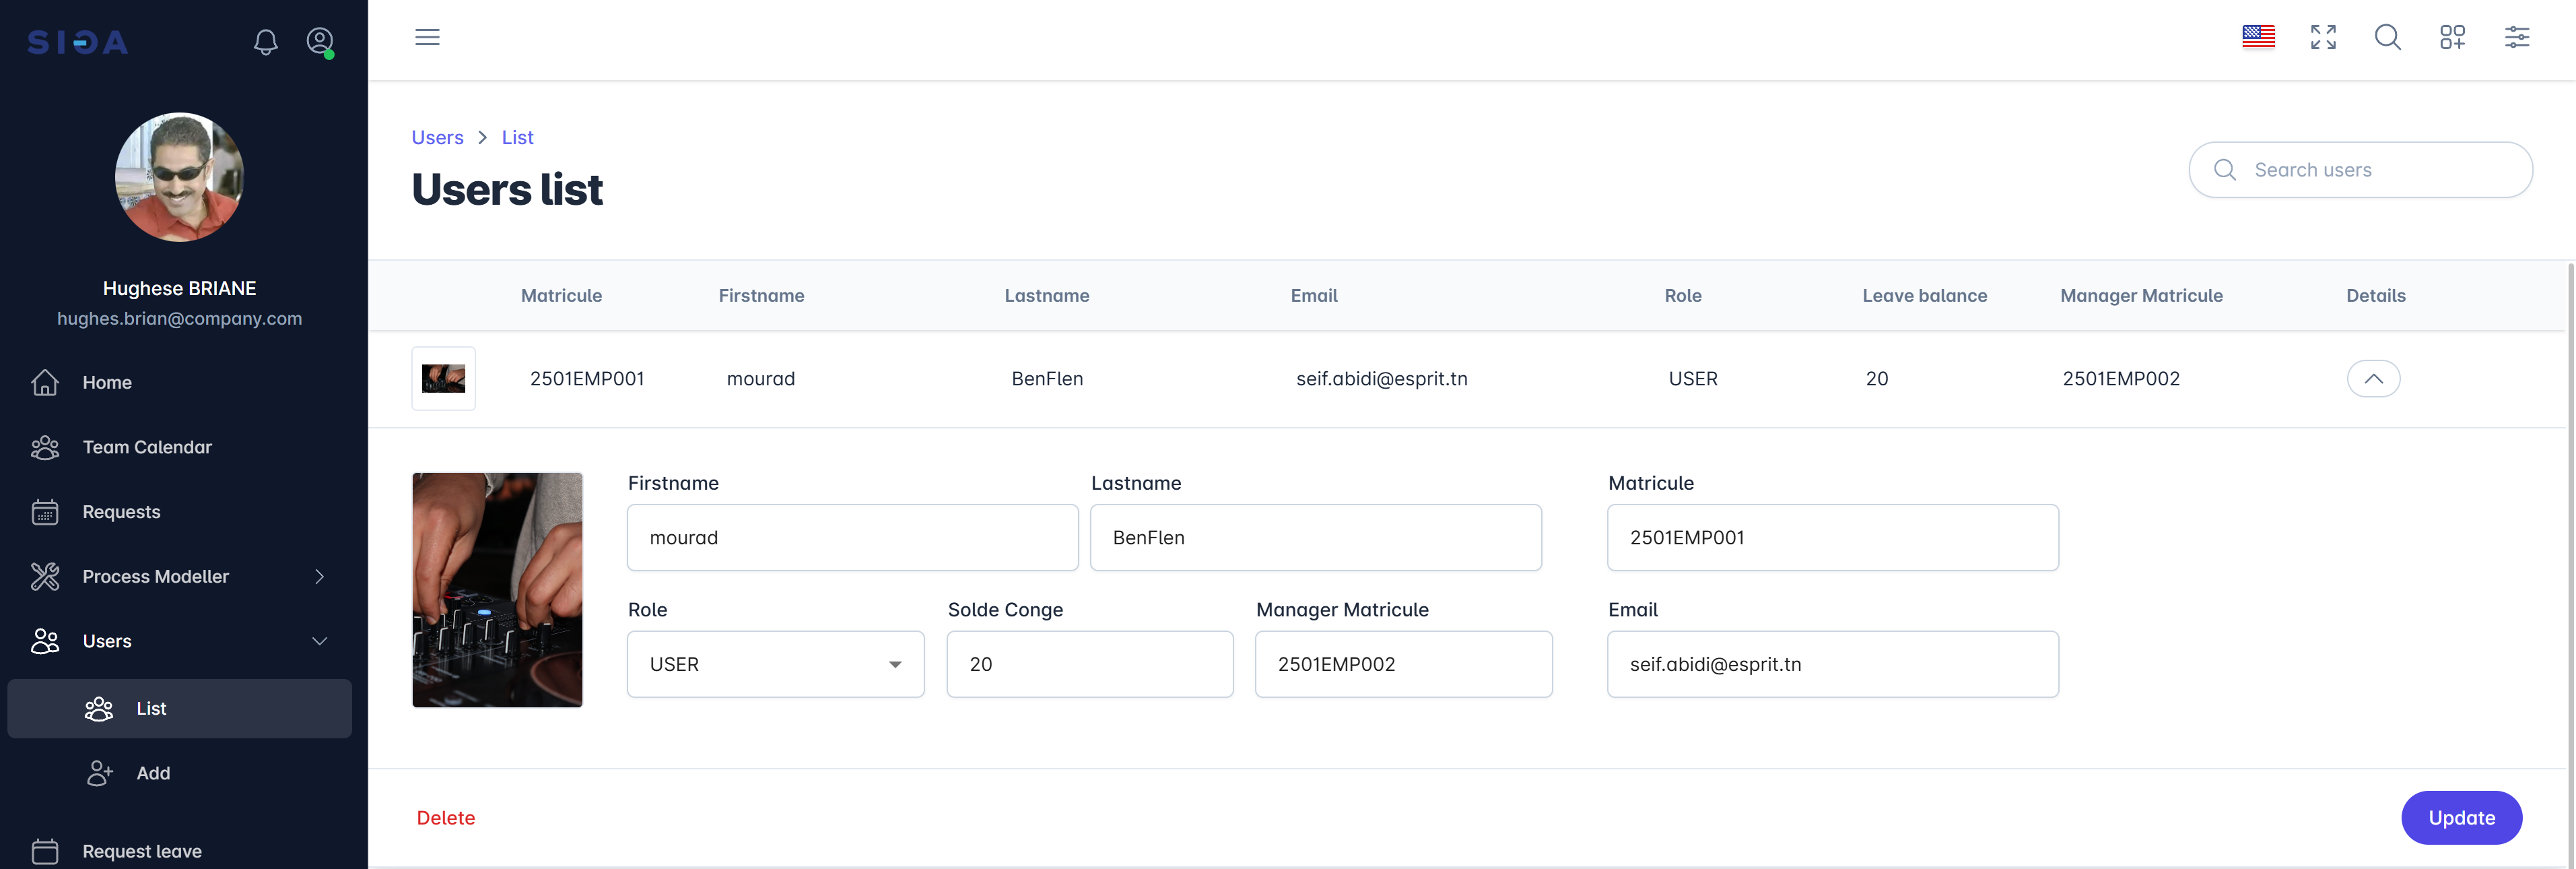
\includegraphics[width=16cm]{images/realisation/dUser.png}
     \caption{Interface du cas d'utilisation <<Consulter les détails d'un utilisateur>>}
     \label{fig:userdetails}
\end{figure}
\newpage
\subsubsection{Modifier un utilisateur}
L’administrateur peut modifier les informations d’un compte existant en accédant à son profil depuis la liste des utilisateurs, comme le montre la figure \ref{fig:edituser}. Une fois les champs mis à jour (nom, e-mail, rôle, etc.), il peut enregistrer les modifications pour qu’elles soient prises en compte immédiatement.
\begin{figure}[H]
     \centering
     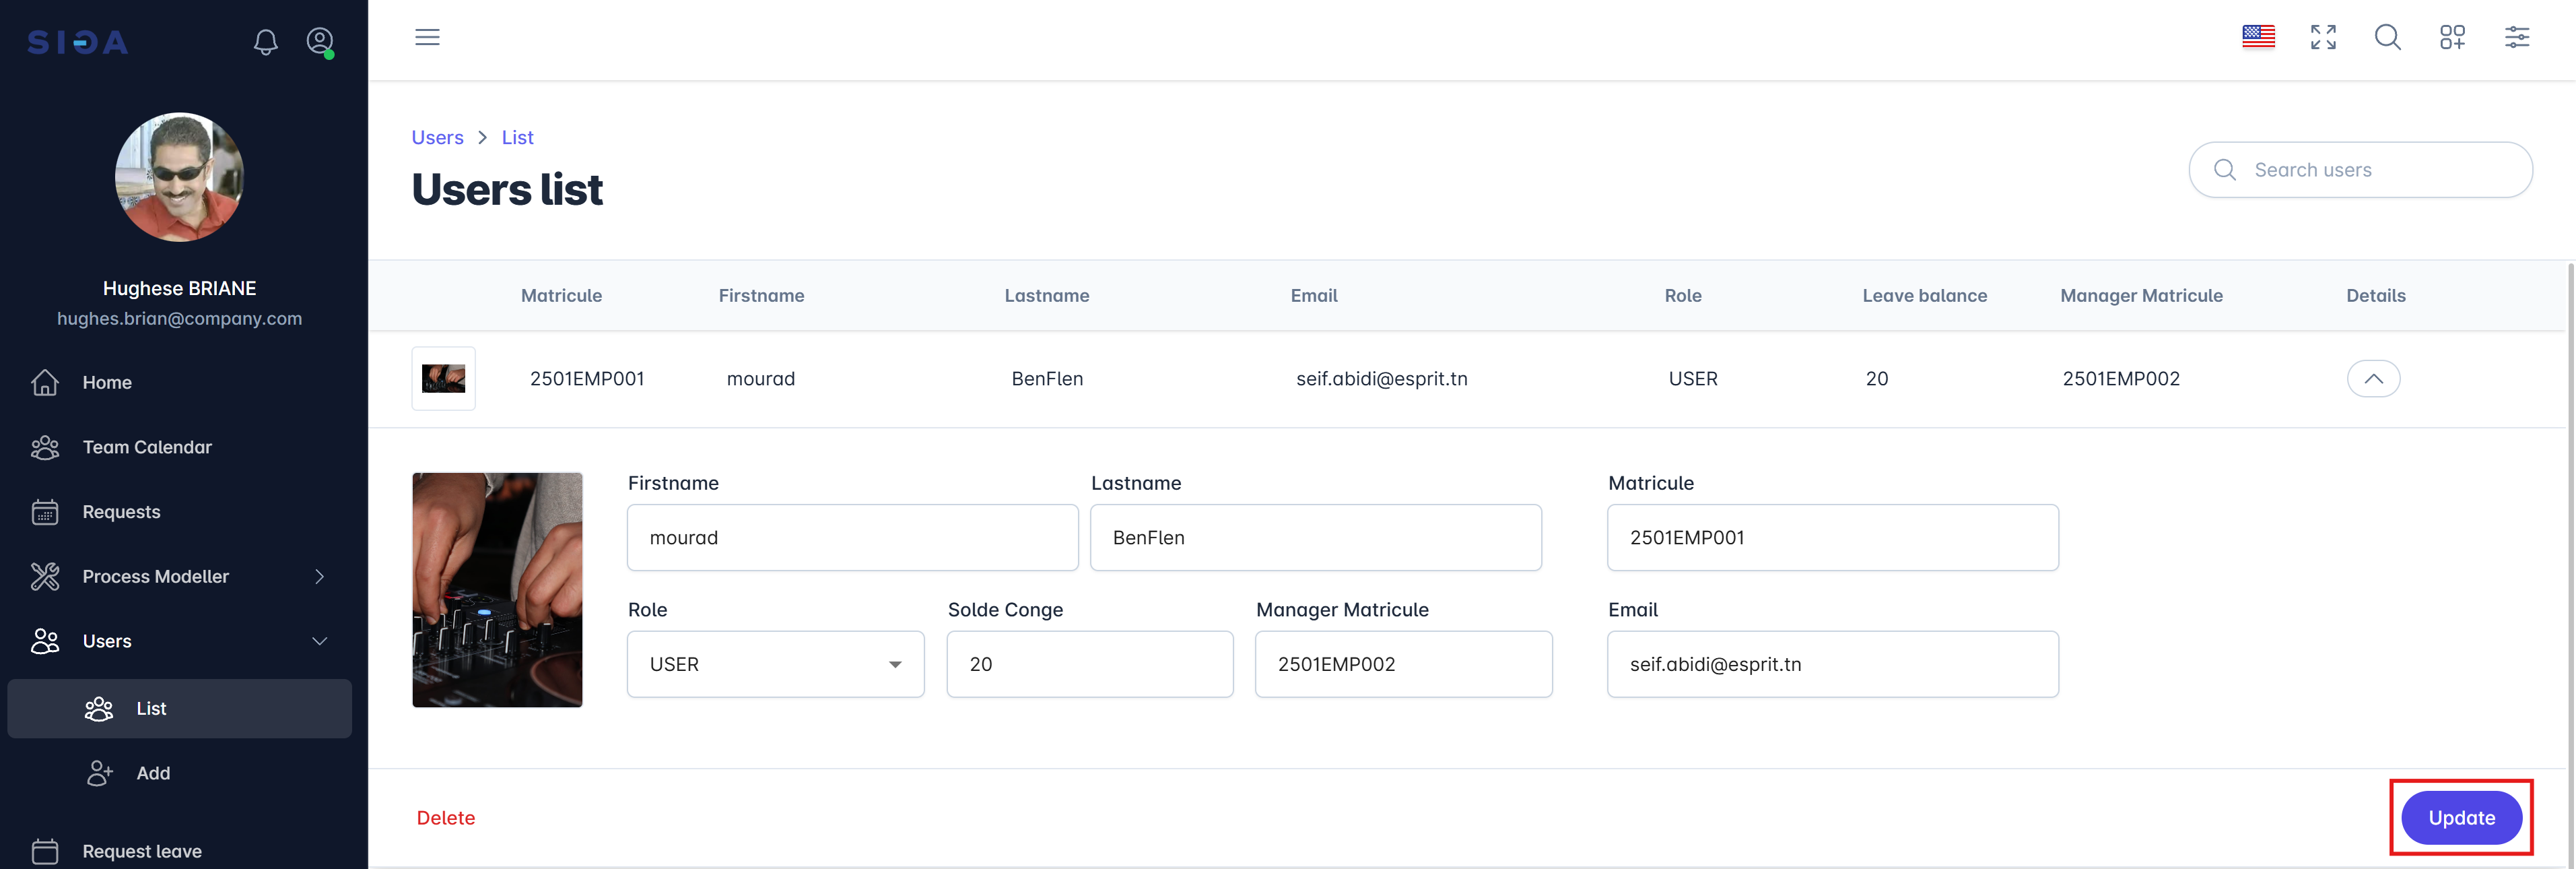
\includegraphics[width=16cm]{images/realisation/mUser.png}
     \caption{Interface du cas d'utilisation <<Modifier un utilisateur>>}
     \label{fig:edituser}
\end{figure}
\subsubsection{Supprimer un utilisateur}
L’administrateur peut supprimer un compte utilisateur en accédant à la liste des utilisateurs et en sélectionnant l’option de suppression associée, comme illustré dans la figure \ref{fig:deleteuser}. Une confirmation est demandée avant la suppression définitive afin d’éviter toute action involontaire.
\begin{figure}[H]
     \centering
     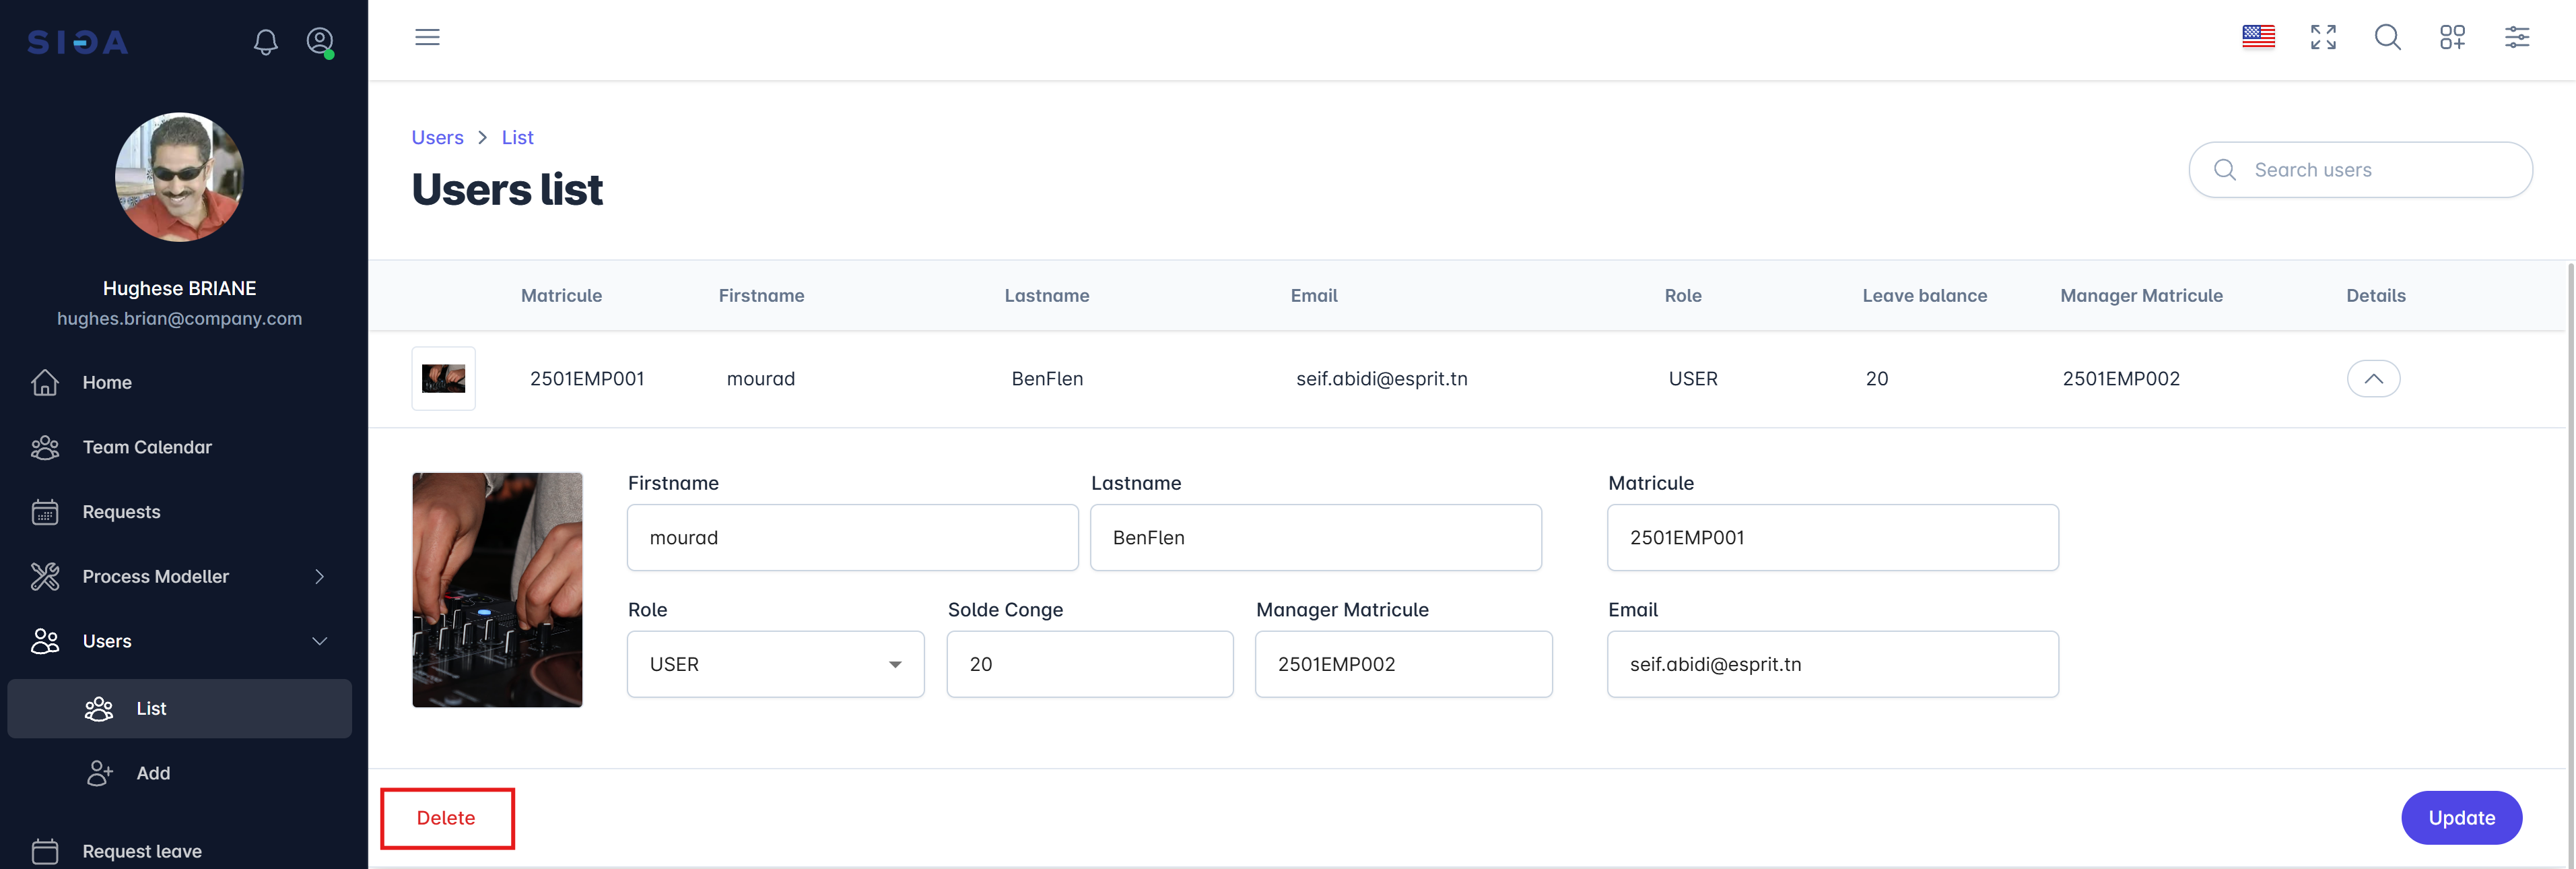
\includegraphics[width=16cm]{images/realisation/sUser.png}
     \caption{Interface du cas d'utilisation <<Supprimer un utilisateur>>}
     \label{fig:deleteuser}
\end{figure}
\newpage
\subsubsection{Intégrer Camunda}
Afin d’intégrer le moteur de workflow Camunda au projet, l’utilisateur doit ajouter les dépendances nécessaires dans le fichier pom.xml, comme illustré dans la figure \ref{fig:camunda-dependencies}. Ces dépendances permettent d’activer le moteur BPM, l’interface web de gestion, ainsi que l’accès aux API REST de Camunda.
\begin{figure}[H]
     \centering
     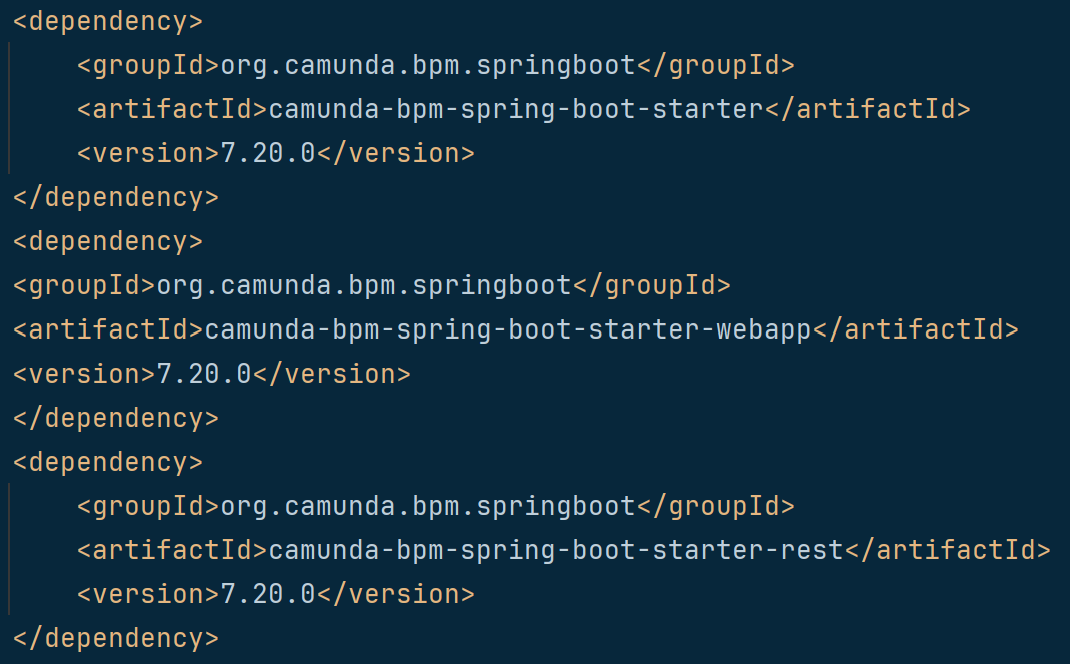
\includegraphics[width=11cm]{images/realisation/cam.png}
     \caption{Interface d'intégration de Camunda}
     \label{fig:camunda-dependencies}
\end{figure}
\subsubsection{Configurer Camunda}
Après avoir ajouté les dépendances nécessaires, l’utilisateur doit configurer Camunda dans le fichier application.properties, comme montré dans la figure \ref{fig:camunda-config}. Cette configuration permet de personnaliser des paramètres essentiels tels que l’authentification, l’accès à l’interface web ou encore le comportement du moteur de workflow au démarrage.
\begin{figure}[H]
     \centering
     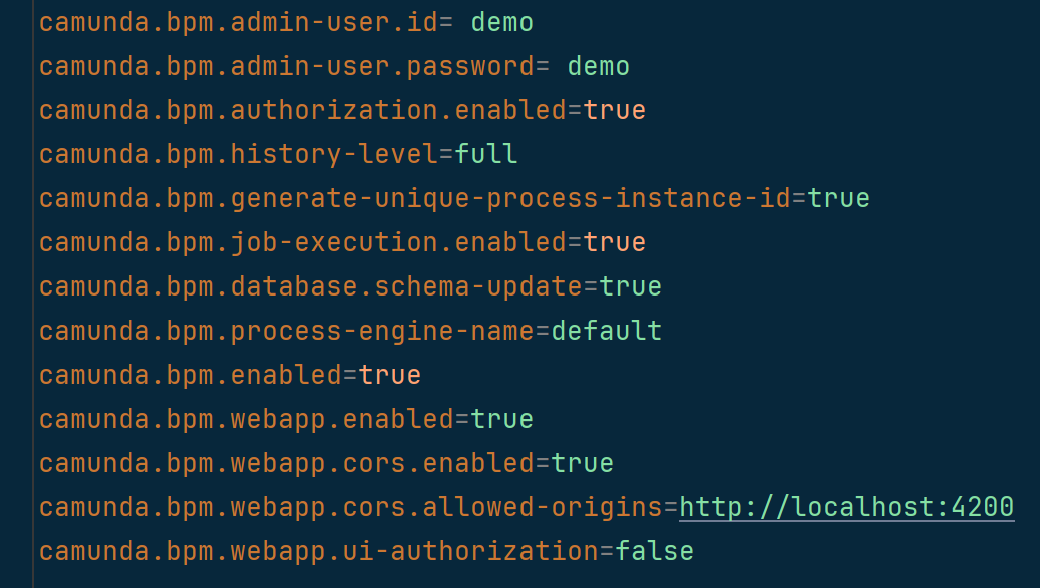
\includegraphics[width=11cm]{images/realisation/camm.png}
     \caption{Interface de configuration de Camunda}
     \label{fig:camunda-config}
\end{figure}
\newpage
\subsubsection{Interface de Camunda}
Une fois l’application démarrée, l’utilisateur ayant les droits appropriés peut accéder à l’interface Cockpit de Camunda, comme illustré dans la figure \ref{fig:camunda-cockpit}. Cette interface web permet de surveiller les processus en cours d’exécution, d’examiner les incidents, et d’analyser les performances du moteur BPMN en temps réel.
\begin{figure}[H]
     \centering
     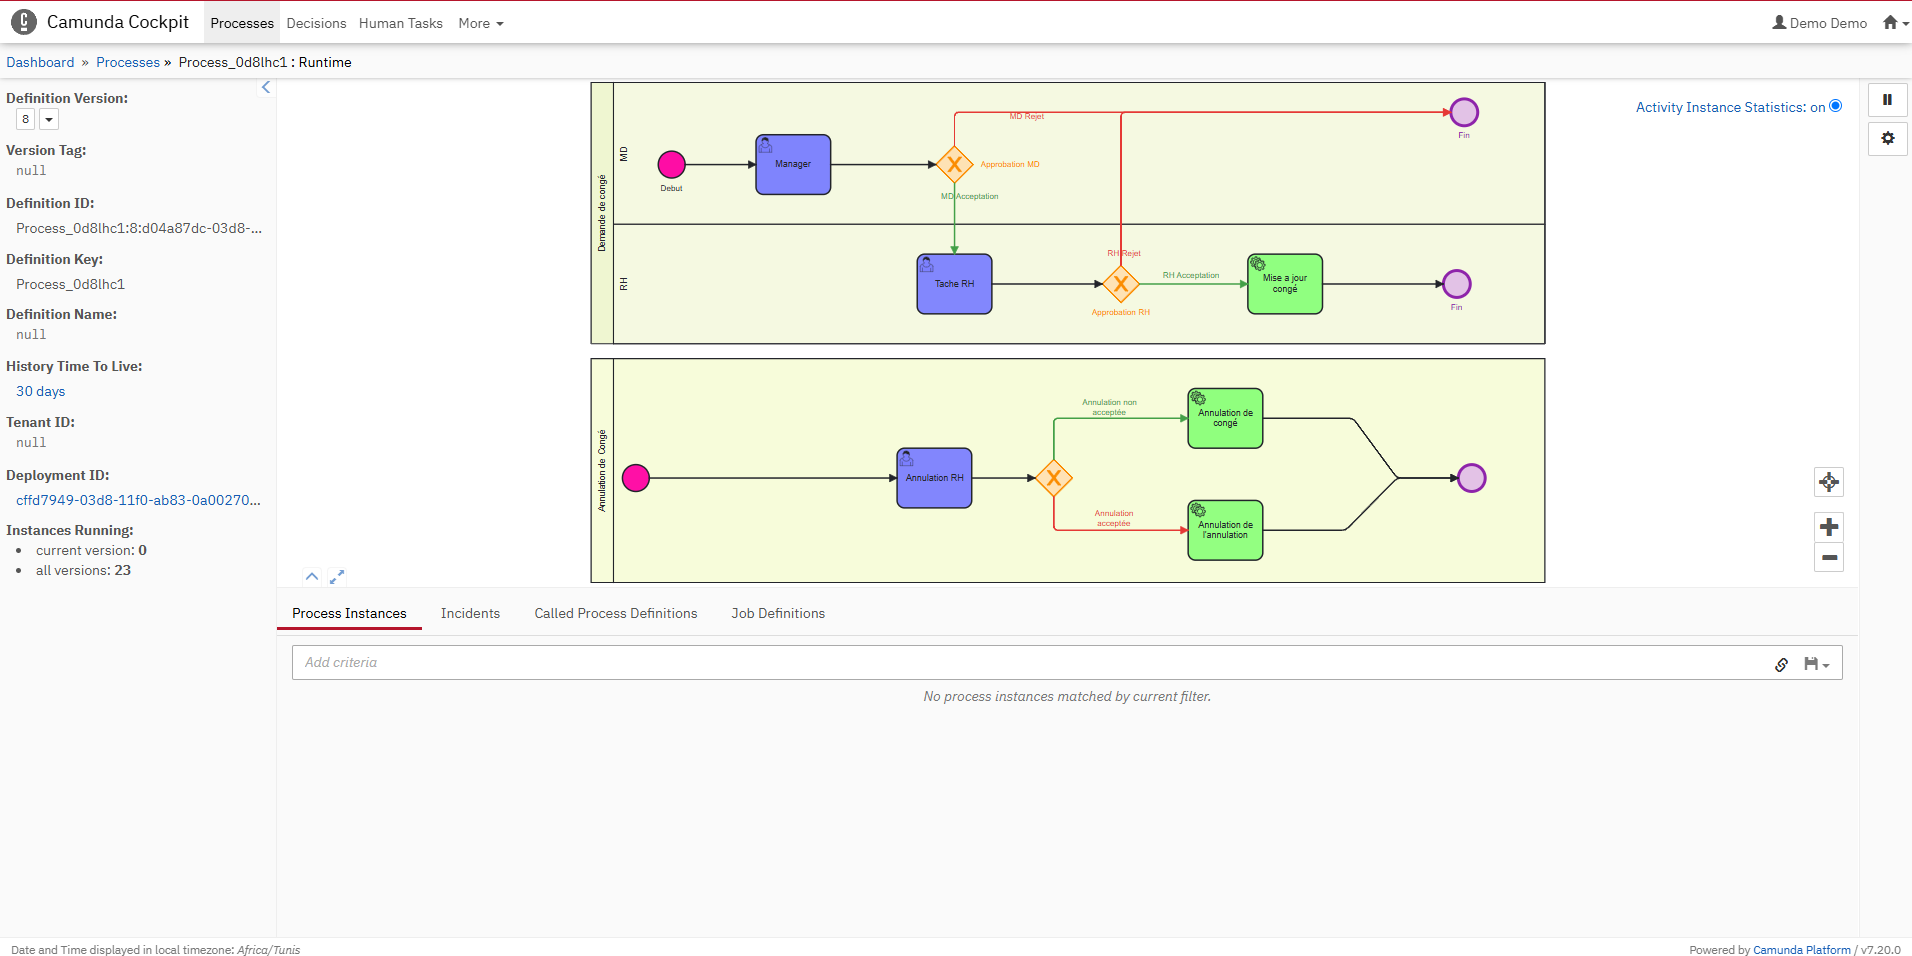
\includegraphics[width=15cm]{images/realisation/pit.png}
     \caption{Interface cockpit de Camunda}
     \label{fig:camunda-cockpit}
\end{figure}
\section{Conclusion}

Le premier sprint du projet a permis de poser des bases solides pour la gestion des accès et l'administration de la plateforme. En implémentant les fonctionnalités clés d'authentification, de déconnexion, de gestion des utilisateurs et d'intégration de Camunda, nous avons établi une infrastructure robuste et sécurisée, essentielle pour les sprints futurs. Les cas d'utilisation ont été soigneusement raffinés, conçus et réalisés, avec des interfaces utilisateur intuitives et des mécanismes techniques fiables, tels que l'utilisation des tokens JWT pour l'authentification, renforcés par les adresses IP des clients et les informations du client-agent (navigateur) pour ajouter une couche supplémentaire de sécurité. L'intégration du moteur de workflow Camunda a également permis de structurer et gérer les processus de manière fluide et évolutive.\\

Cette étape a non seulement répondu aux besoins fonctionnels prioritaires, mais a également renforcé la qualité, la sécurité et la fiabilité du système grâce à des pratiques de développement rigoureuses. Les fondations établies dans ce sprint garantiront une évolutivité et une maintenabilité optimales pour les prochaines itérations du projet.







 


 


 

